\documentclass{article}
\usepackage[T1]{fontenc}
\usepackage[polish]{babel}
\usepackage{amssymb}
\usepackage{amsmath}
\usepackage{graphicx}
\usepackage{subcaption}
\usepackage{booktabs}
\usepackage[section]{placeins}

\title{Implementacja sieci neuronowej MLP i ewaluacja w zadaniach klasyfikacji i regresji}
\author{Hubert Błonowski \and Jan Zaborski}
\date{}

\begin{document}

\maketitle

\begin{abstract}
Zaimplementowaliśmy od podstaw perceptron wielowarstwowy (MLP) uczony metodą propagacji wstecznej
i stochastycznego spadku gradientu. Na dwóch zbiorach do klasyfikacji punktów na płaszczyźnie
i dwóch zbiorach do regresji funkcji jednej zmiennej zbadaliśmy wpływ funkcji aktywacji, liczby
i szerokości warstw ukrytych, funkcji kosztu oraz biasów na jakość uczenia. Każdą konfigurację uczono
z pięcioma ziarnami losowymi. Tę samą implementację zastosowaliśmy do rozpoznawania cyfr ze zbioru
MNIST, osiągając 98,3\% trafności na zbiorze testowym siecią z dwiema warstwami ukrytymi po 512
neuronów.
\end{abstract}

\tableofcontents

\section{Wstęp}

Rozważamy dwa podstawowe zadania uczenia nadzorowanego, klasyfikację i regresję.

Celem projektu jest implementacja sieci MLP do obu zadań, wizualizacja jej działania i uczenia oraz
zbadanie, jak na wyniki wpływają funkcja aktywacji, architektura sieci i funkcja kosztu. W części
pierwszej korzystamy z małych zbiorów danych w~$\mathbb{R}^2$ (klasyfikacja) i~$\mathbb{R}$
(regresja), które pozwalają łatwo zwizualizować, czego nauczyła się sieć. W części drugiej tę samą
implementację stosujemy do zbioru MNIST.

Rozdział~\ref{sec:teoria} krótko omawia ideę sieci MLP i ich uczenia, rozdział~\ref{sec:impl} naszą
implementację, a rozdział~\ref{sec:procedura} procedurę eksperymentalną. Wyniki dla małych zbiorów
przedstawia rozdział~\ref{sec:wyniki}, dla MNIST rozdział~\ref{sec:mnist}. Szczegółowe wzory
pomijamy, odsyłając do literatury.

\section{Podstawy teoretyczne}
\label{sec:teoria}

Podstawowym elementem sieci MLP (\emph{Multi-Layer Perceptron}) jest neuron o wejściach
$x_1, \ldots, x_n$, wagach $w_1, \ldots, w_n$, biasie $b$ i funkcji aktywacji $f$, obliczający
$y = f(\sum_{i=1}^{n} w_i x_i + b)$. Neurony przetwarzające to samo wejście tworzą warstwę
(zakładamy, że mają wspólną funkcję aktywacji). Sieć składa się z warstw ukrytych i warstwy
wyjściowej, przy czym wejściem każdej warstwy jest wyjście poprzedniej, a obliczenie predykcji przez
kolejne warstwy nazywamy przejściem w przód (\emph{forward pass}).

Funkcje aktywacji warstw ukrytych (np.\ sigmoida, $\tanh$, ReLU) muszą być nieliniowe, bo złożenie
przekształceń liniowych jest liniowe i głębsza sieć nie dawałaby nic więcej niż jedna warstwa.
W warstwie wyjściowej stosuje się identyczność w regresji oraz softmax w klasyfikacji, zwracający
prawdopodobieństwa przynależności do każdej z klas.

Jakość predykcji $\hat{y}$ względem wartości prawdziwej $y$ mierzy funkcja kosztu
$\mathcal{L}(y, \hat{y})$, np.\ błąd średniokwadratowy (MSE) lub średni błąd bezwzględny (MAE)
w regresji oraz entropia krzyżowa w klasyfikacji. Uczenie polega na minimalizacji średniego kosztu
na zbiorze uczącym metodą spadku gradientu: wagi i biasy są wielokrotnie przesuwane o mały krok
(współczynnik uczenia) w kierunku przeciwnym do gradientu kosztu. W wersji stochastycznej (SGD)
gradient liczy się na małych, losowych porcjach danych (\emph{mini-batch}), co pozwala wykonać
znacznie więcej kroków w tym samym czasie. Wagi inicjalizuje się losowo, aby neurony jednej warstwy
nie uczyły się identycznie.

Gradient względem wszystkich parametrów wyznacza algorytm propagacji wstecznej
(\emph{backpropagation}), oparty na regule łańcuchowej: błąd $\delta = \partial\mathcal{L}/\partial z$
liczony względem wejść neuronów wyjściowych (przed aktywacją) jest przekazywany warstwa po warstwie
w stronę wejścia, a w każdej warstwie wyznacza się z niego gradienty jej wag.

Wszystkie te operacje można zapisać w języku algebry liniowej. Wagi warstwy tworzą macierz, a porcja
danych macierz, której wiersze są przykładami; przejście w przód przez warstwę jest wtedy jednym
mnożeniem macierzy, a propagacja wsteczna sprowadza się do mnożeń przez macierze transponowane.
Mnożenie macierzy wykonuje dużo obliczeń na każdej wczytanej liczbie, dzięki czemu dobrze
wykorzystuje pamięć podręczną, instrukcje wektorowe procesora (SIMD) i karty graficzne.

\section{Implementacja sieci}
\label{sec:impl}

Sieć oraz wszystkie operacje na macierzach zaimplementowano od podstaw w języku Rust, bez bibliotek
uczenia maszynowego i algebry liniowej. Jedyną zewnętrzną zależnością biblioteki jest generator liczb
losowych. Rust wybrano ze względu na niskopoziomową kontrolę nad układem danych i obliczeniami,
wygodną składnię oraz automatyczną wektoryzację kodu przez kompilator. W kodzie nie używano jawnych
instrukcji SIMD ani wielowątkowości, mimo to wydajność jest zadowalająca: epoka uczenia na MNIST trwa
od ok.\ 1\,s (sieć 784--128--10) do ok.\ 10\,s (784--512--512--10), wliczając ewaluację na zbiorach
uczącym i testowym.

Macierze przechowywane są wierszowo (row-major), a porcja danych jest macierzą, której wiersze są
przykładami. Warstwa liczy więc $Z = XW + b$, gdzie $W$ ma wymiary
\emph{wejścia}~$\times$~\emph{neurony}, czyli jest transpozycją macierzy wag z
typowego zapisu w literaturze. Układ ten zapewnia ciągły dostęp do pamięci zarówno przy przetwarzaniu
przykładów, jak i wierszy wag.

Sieć to lista warstw (macierz wag i opcjonalny wektor biasów) wraz ze wspólną funkcją aktywacji
warstw ukrytych oraz funkcją aktywacji wyjścia połączoną z funkcją kosztu. Przejście w przód
składa się z mnożenia macierzy (GEMM), dodania biasu do każdego wiersza i zastosowania funkcji
aktywacji dla każdego elementu. Wyniki pośrednie zapisywane są w przydzielanej raz pamięci roboczej
i wykorzystywane podczas propagacji wstecznej. Gradienty wag i błąd przekazywany do poprzedniej
warstwy liczone są wariantami GEMM, które traktują jeden z argumentów jako transponowany, więc
transpozycji nie trzeba tworzyć w pamięci. Wagi inicjalizowane są losowo metodą
Xaviera~\cite{glorot2010} (dla ReLU metodą He~\cite{he2015}), biasy zerami, a wejścia są
normalizowane statystykami zbioru uczącego.

Każdy eksperyment opisuje plik JSON z danymi, architekturą (lista szerokości warstw ukrytych,
obecność biasów, funkcja aktywacji, funkcja kosztu), parametrami uczenia i listą ziaren. Ziarno
inicjalizuje generator, z którego losowane są wagi początkowe i kolejność przykładów w każdej epoce,
więc uczenie z tym samym plikiem i ziarnem jest w pełni powtarzalne. Program zapisuje konfigurację
razem z wynikami, a dla każdego ziarna: wartości kosztu i metryk w każdej epoce, predykcje
na zbiorze testowym (dla danych jedno- i dwuwymiarowych) oraz opcjonalnie wagi wszystkich warstw i sygnały $\delta$ propagowane wstecz
dla ustalonego przykładu uczącego. Na tej podstawie skrypty w Pythonie rysują wykresy z
rozdziałów~\ref{sec:wyniki}--\ref{sec:mnist}.

\section{Procedura eksperymentalna}
\label{sec:procedura}

\paragraph{Zbiory danych.} Zbiory \emph{simple} i \emph{three\_gauss} zawierają punkty
płaszczyzny podzielone odpowiednio na 2 i 3 klasy; w \emph{simple} klasy są rozdzielone prawie
liniowo, a w \emph{three\_gauss} pochodzą z trzech częściowo nakładających się rozkładów normalnych.
Zbiory \emph{cube} i \emph{activation} zawierają próbki funkcji $\mathbb{R}\to\mathbb{R}$:
wielomianu stopnia trzeciego i funkcji o kształcie esowatym. W obu zbiorach regresyjnych punkty
testowe pokrywają szerszy przedział $x$ niż uczące (tab.~\ref{tab:dane}), dlatego błąd testowy
liczymy osobno dla punktów z zakresu danych uczących (interpolacja) i spoza niego (ekstrapolacja).
Zbiór MNIST opisuje rozdział~\ref{sec:mnist}.

\begin{table}[htbp]
\centering
\resizebox{\linewidth}{!}{%
\begin{tabular}{lcccc}
\toprule
 & \emph{simple} & \emph{three\_gauss} & \emph{cube} & \emph{activation} \\
\midrule
zadanie & \multicolumn{2}{c}{klasyfikacja w $\mathbb{R}^2$} & \multicolumn{2}{c}{regresja $\mathbb{R}\to\mathbb{R}$} \\
liczba klas / wyjść & 2 & 3 & 1 & 1 \\
przykłady: uczące / testowe & 1000 / 1000 & 1000 / 1000 & 1000 / 1000 & 1000 / 1000 \\
zakres $x$: uczący / testowy & --- & --- & $[-2, 4]$ / $[-5, 5]$ & $[-4, 4]$ / $[-5, 5]$ \\
test w zakresie / poza zakresem & --- & --- & 599 / 401 & 796 / 204 \\
\bottomrule
\end{tabular}}
\caption{Zbiory danych części pierwszej.}
\label{tab:dane}
\end{table}

\paragraph{Plan badań.} Każde badanie zmienia jeden czynnik względem konfiguracji bazowej
(tab.~\ref{tab:baseline}):
\begin{itemize}
  \item architekturę: liczbę warstw ukrytych $L \in \{0,\dots,4\}$ i liczbę neuronów w warstwie
  $B \in \{4, 8, 16, 32, 64\}$ (wszystkie kombinacje),
  \item funkcję aktywacji warstw ukrytych: sigmoida, $\tanh$, ReLU,
  \item funkcję kosztu: entropia krzyżowa i MSE (na wyjściu softmax) dla klasyfikacji, MSE i MAE
  dla regresji,
  \item obecność biasów, dla sieci $1\times8$ i $2\times32$.
\end{itemize}
Ponieważ najlepszy współczynnik uczenia zależy od funkcji aktywacji i kosztu, oba te badania
powtórzono dla współczynników $\{0{,}003;\ 0{,}01;\ 0{,}03;\ 0{,}1;\ 0{,}3;\ 1\}$.

\paragraph{Ocena.} Sieć uczy się na
całym zbiorze uczącym przez stałą liczbę epok, a zbiór testowy jest oceniany po każdej epoce
wyłącznie w celu zapisu wyników. Mierzymy trafność (accuracy) i macro-F1 w klasyfikacji oraz MSE
i MAE (w oryginalnych jednostkach $y$) w regresji. Ponieważ przy stałym współczynniku uczenia
wynik waha się między epokami, jako wynik końcowy przyjmujemy średnią z ostatnich 50 epok.
Każdą konfigurację uczymy z 5 ziarnami (0--4) i podajemy medianę oraz rozstęp międzykwartylowy (IQR).
Przebiegi, w których uczenie się rozbiegło (wartości nieskończone), pomijamy w statystykach
i zaznaczamy na wykresach symbolem $\times n$, gdzie $n$ to liczba takich ziaren.

\begin{table}[htbp]
\centering
\resizebox{\linewidth}{!}{%
\begin{tabular}{lcc}
\toprule
 & klasyfikacja & regresja \\
\midrule
warstwy ukryte $L \times B$ & \multicolumn{2}{c}{$2 \times 32$} \\
aktywacja warstw ukrytych & \multicolumn{2}{c}{$\tanh$} \\
wyjście i funkcja kosztu & softmax, entropia krzyżowa & liniowe, MSE \\
biasy / inicjalizacja & \multicolumn{2}{c}{tak / Xavier, biasy zerowe} \\
optymalizator & \multicolumn{2}{c}{mini-batch SGD, stały współczynnik 0,1, batch 32} \\
liczba epok & 260 (\emph{simple}), 340 (\emph{three\_gauss}) & 1000 \\
normalizacja & wejścia: standaryzacja & wejścia i wyjście: standaryzacja \\
precyzja obliczeń & \multicolumn{2}{c}{64-bitowa} \\
\bottomrule
\end{tabular}}
\caption{Konfiguracja bazowa części pierwszej. Każde badanie zmienia jeden z czynników,
pozostałe pozostają bez zmian.}
\label{tab:baseline}
\end{table}

\section{Wyniki: klasyfikacja w $\mathbb{R}^2$ i regresja $\mathbb{R}\to\mathbb{R}$}
\label{sec:wyniki}

\subsection{Wizualizacja uczenia}

Rysunek~\ref{fig:klasyfikacja} przedstawia obszary decyzyjne sieci bazowej i jej pomyłki na zbiorze
testowym.
Rysunek~\ref{fig:regresja} pokazuje funkcje nauczone w regresji: w zakresie danych uczących sieć
pokrywa się z funkcją docelową, a poza nim jej przebieg zależy od funkcji aktywacji.

\begin{figure}[htbp]
  \centering
  \begin{subfigure}{0.32\linewidth}
    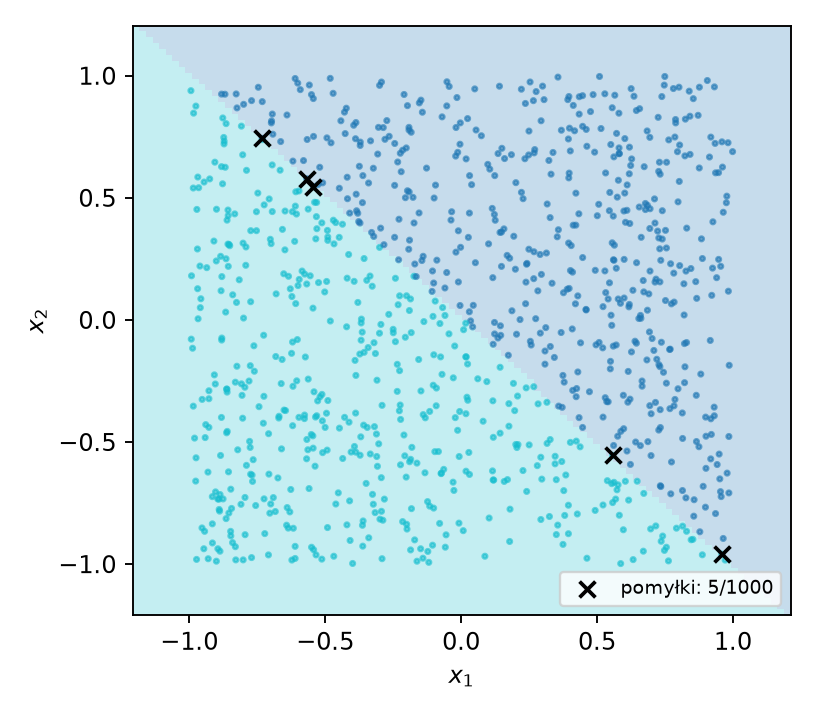
\includegraphics[width=\linewidth]{figures/simple/predictions_tanh.png}
    \caption{\emph{simple}}
  \end{subfigure}\hfill
  \begin{subfigure}{0.32\linewidth}
    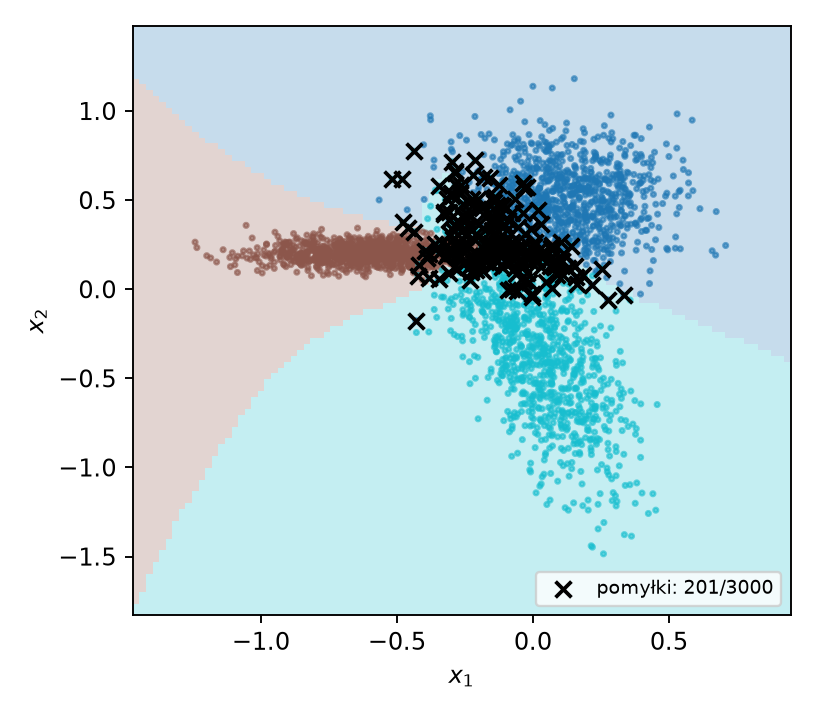
\includegraphics[width=\linewidth]{figures/three_gauss/predictions_tanh.png}
    \caption{\emph{three\_gauss}}
  \end{subfigure}\hfill
  \begin{subfigure}{0.32\linewidth}
    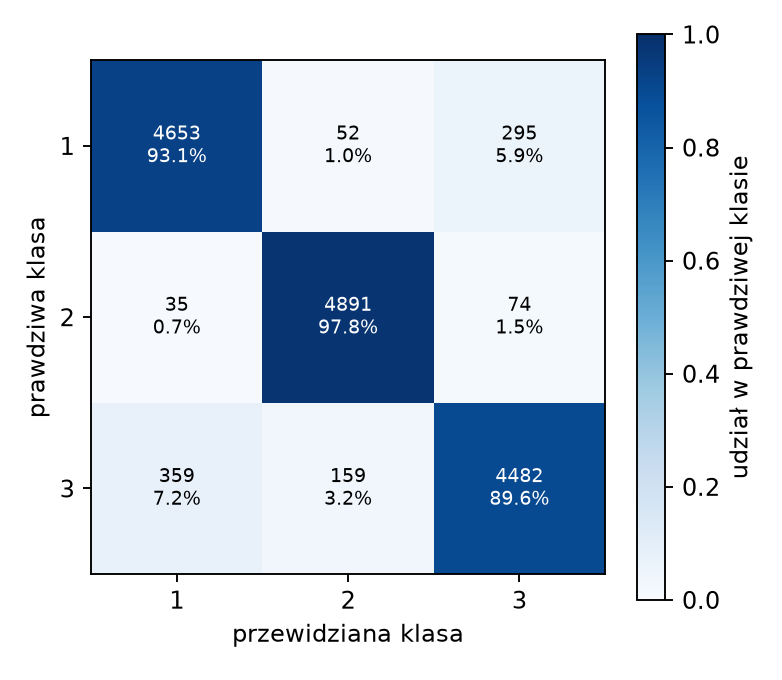
\includegraphics[width=\linewidth]{figures/three_gauss/confusion_tanh_32x32.png}
    \caption{\emph{three\_gauss}}
  \end{subfigure}
  \caption{Klasyfikacja siecią bazową nauczoną z ziarnem 0. (a), (b): kolor tła -- klasa przewidziana
  przez sieć w punktach siatki $100\times100$ pokrywającej zakres danych uczących; punkty -- zbiór
  testowy w kolorze prawdziwej klasy, $\times$ -- punkt testowy sklasyfikowany błędnie.
  (c): macierz pomyłek na zbiorze testowym zsumowana po 5 ziarnach.}
  \label{fig:klasyfikacja}
\end{figure}

\begin{figure}[htbp]
  \centering
  \begin{subfigure}{0.49\linewidth}
    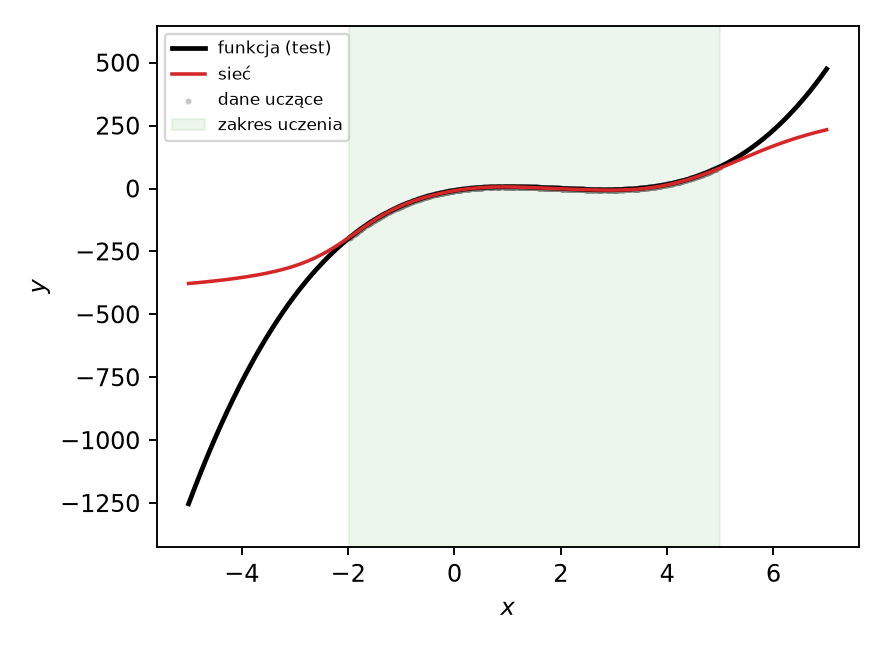
\includegraphics[width=\linewidth]{figures/cube/predictions_tanh.png}
    \caption{\emph{cube}, $\tanh$}
  \end{subfigure}\hfill
  \begin{subfigure}{0.49\linewidth}
    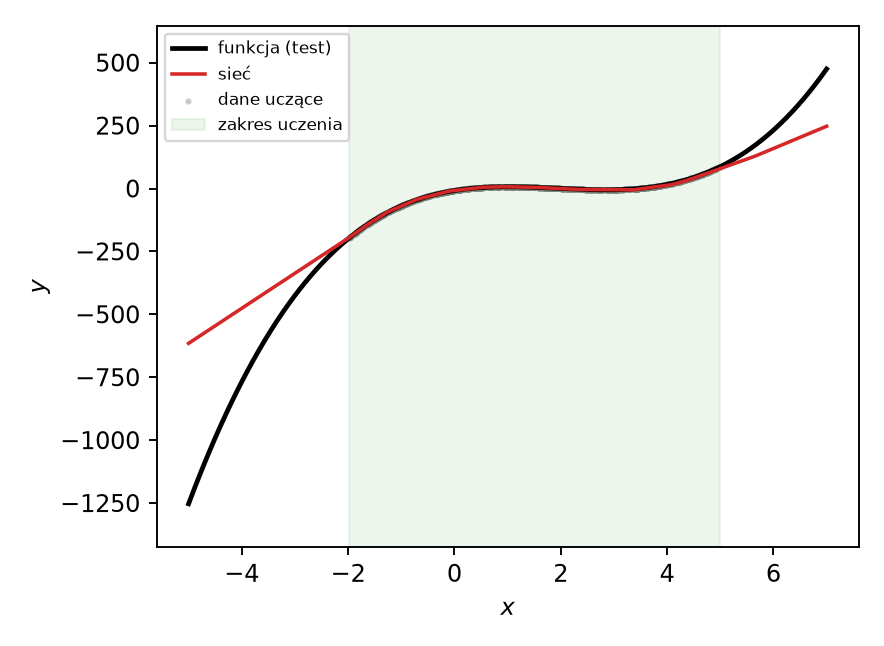
\includegraphics[width=\linewidth]{figures/cube/predictions_relu.png}
    \caption{\emph{cube}, ReLU}
  \end{subfigure}
  \begin{subfigure}{0.49\linewidth}
    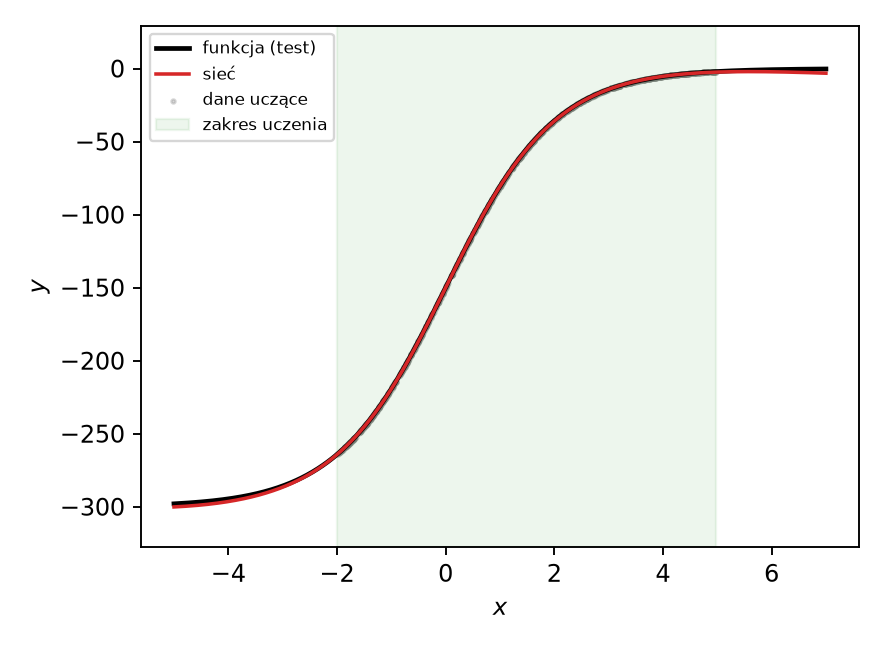
\includegraphics[width=\linewidth]{figures/activation/predictions_tanh.png}
    \caption{\emph{activation}, $\tanh$}
  \end{subfigure}\hfill
  \begin{subfigure}{0.49\linewidth}
    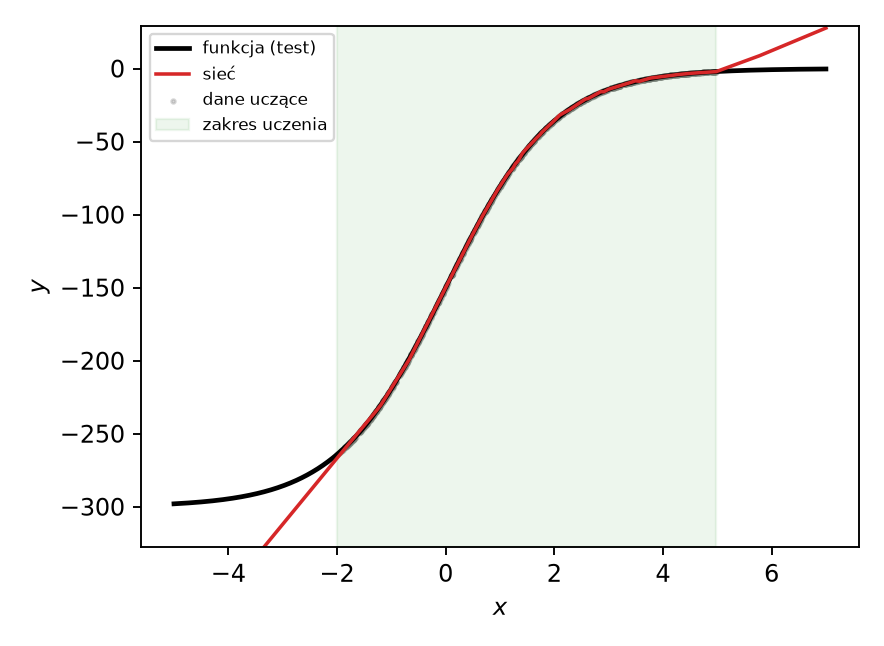
\includegraphics[width=\linewidth]{figures/activation/predictions_relu.png}
    \caption{\emph{activation}, ReLU}
  \end{subfigure}
  \caption{Regresja siecią $2\times32$ (ziarno 0) na całym zakresie zbioru testowego. Zielone tło
  oznacza zakres $x$ danych uczących.}
  \label{fig:regresja}
\end{figure}

Przebieg kosztu w kolejnych epokach przedstawia rys.~\ref{fig:koszt-epoki}. Koszt na zbiorze
testowym przez cały czas uczenia pozostaje blisko kosztu na zbiorze uczącym. Na \emph{simple}
i \emph{cube} koszt wyraźnie oscyluje między epokami.

\begin{figure}[htbp]
  \centering
  \begin{subfigure}{0.49\linewidth}
    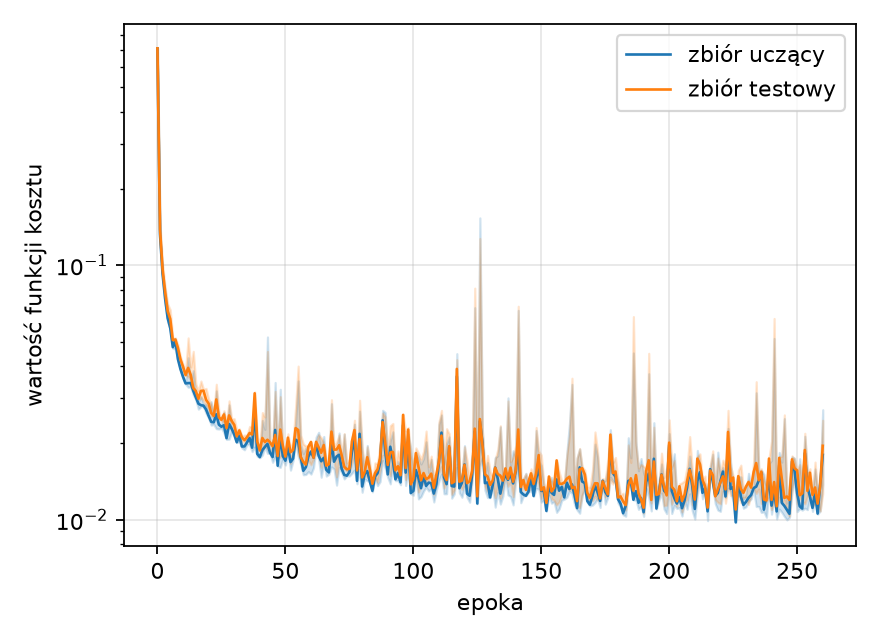
\includegraphics[width=\linewidth]{figures/simple/cost_curve.png}
    \caption{\emph{simple}}
  \end{subfigure}\hfill
  \begin{subfigure}{0.49\linewidth}
    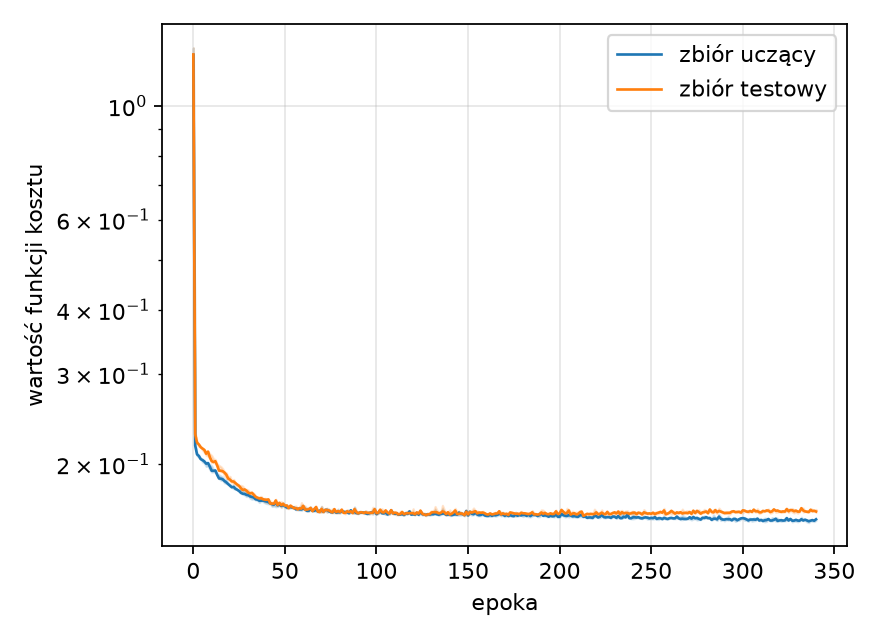
\includegraphics[width=\linewidth]{figures/three_gauss/cost_curve.png}
    \caption{\emph{three\_gauss}}
  \end{subfigure}
  \begin{subfigure}{0.49\linewidth}
    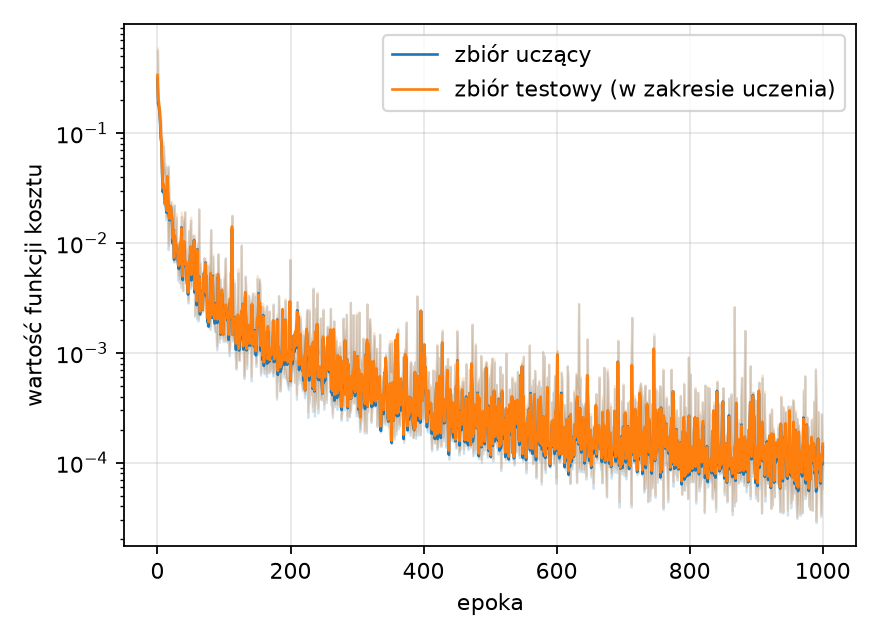
\includegraphics[width=\linewidth]{figures/cube/cost_curve.png}
    \caption{\emph{cube}}
  \end{subfigure}\hfill
  \begin{subfigure}{0.49\linewidth}
    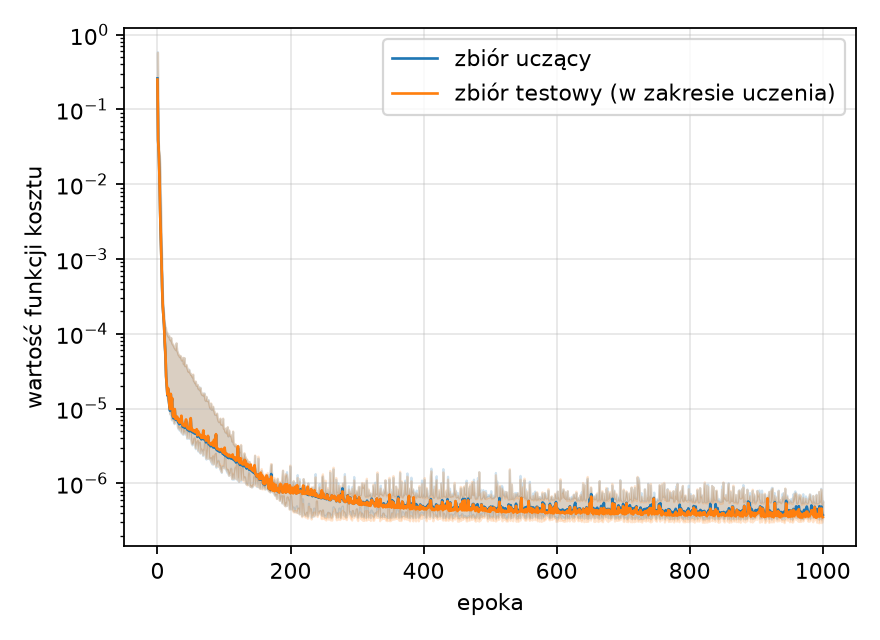
\includegraphics[width=\linewidth]{figures/activation/cost_curve.png}
    \caption{\emph{activation}}
  \end{subfigure}
  \caption{Wartość funkcji kosztu sieci bazowej w kolejnych epokach (mediana i IQR z 5 ziaren).
  W regresji koszt liczony jest dla znormalizowanych wartości $y$.}
  \label{fig:koszt-epoki}
\end{figure}

Ewolucję wag i propagowanego błędu pokazujemy dla mniejszej sieci $2\times8$ na zbiorze \emph{cube}
(rys.~\ref{fig:graf}--\ref{fig:delty}). Wagi zmieniają się najszybciej na początku uczenia,
kiedy najszybciej maleje też koszt. Sygnały $\delta$ we wszystkich warstwach są największe
(do ok.\ 0,6 co do wartości bezwzględnej) w pierwszych kilkudziesięciu epokach, a po ok.\ 400
epokach są bliskie zeru.

\begin{figure}[htbp]
  \centering
  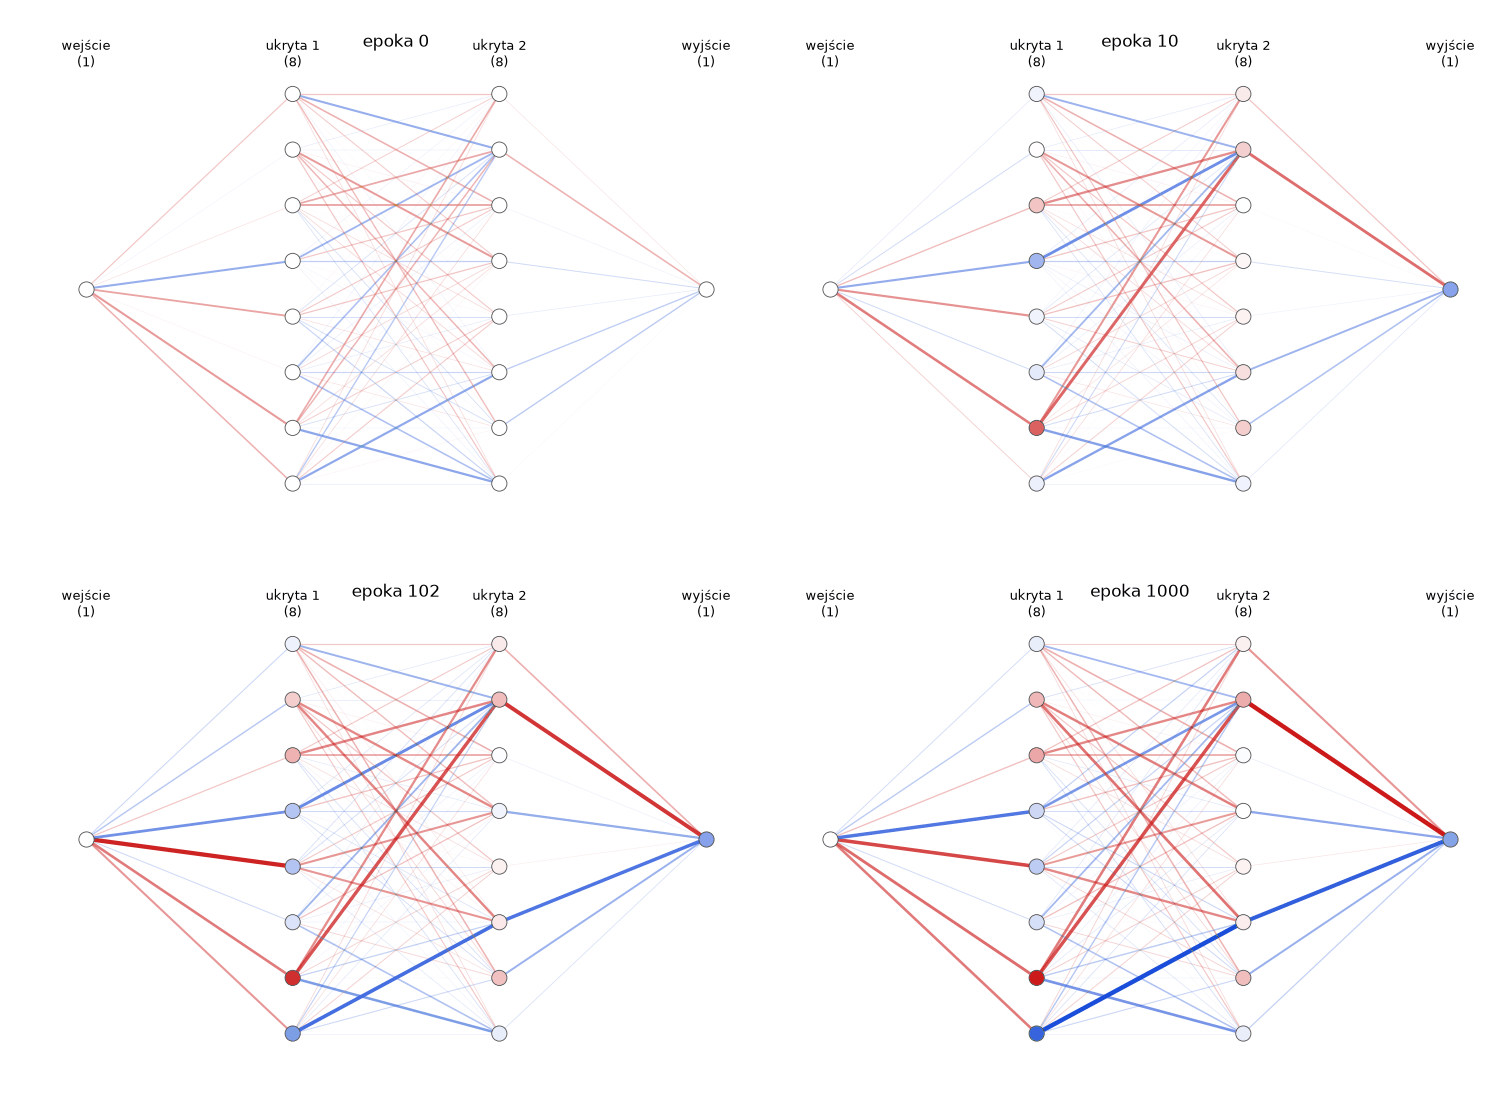
\includegraphics[width=0.9\linewidth]{figures/cube/graph_frames.png}
  \caption{Wagi sieci $2\times8$ (\emph{cube}, ziarno 0) w epokach 0, 10, 100 i 1000. Kolor
  krawędzi to znak wagi (czerwony -- dodatnia, niebieski -- ujemna), grubość i nasycenie --
  jej wartość bezwzględna; wypełnienie neuronu oznacza bias. Każda warstwa ma własną skalę.
  }
  \label{fig:graf}
\end{figure}

\begin{figure}[htbp]
  \centering
  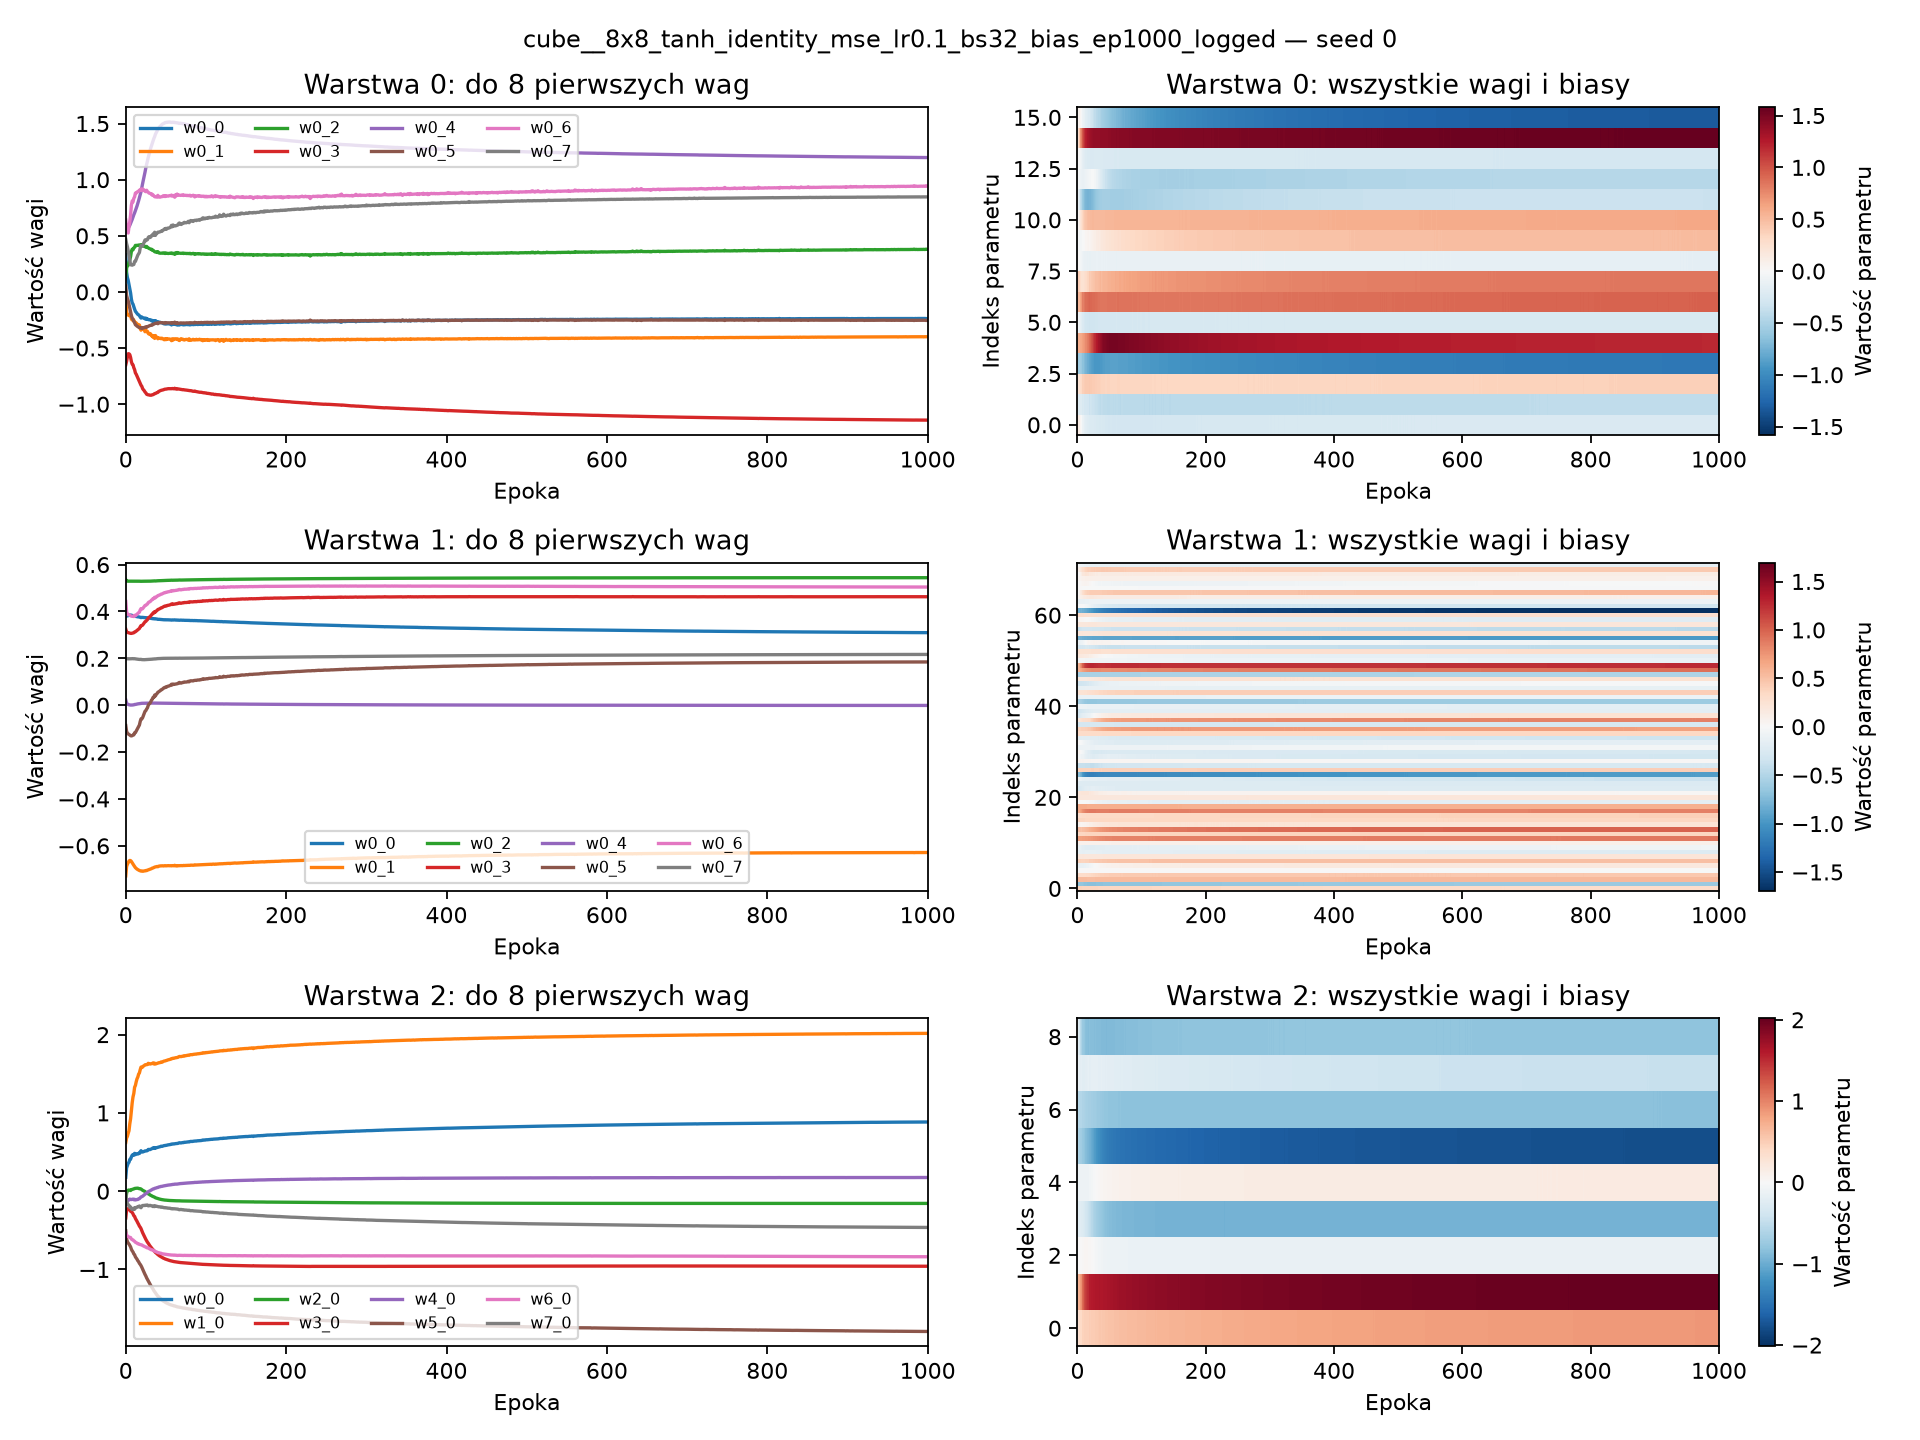
\includegraphics[width=\linewidth]{figures/single/cube__8x8_tanh_identity_mse_lr0.1_bs32_bias_ep1000_logged/seed_0/weights.png}
  \caption{Wartości wag sieci $2\times8$ (\emph{cube}, ziarno 0) po kolejnych epokach. Z lewej
  przebieg 8 wybranych wag każdej warstwy, z prawej wszystkie wagi i biasy warstwy.}
  \label{fig:wagi}
\end{figure}

\begin{figure}[htbp]
  \centering
  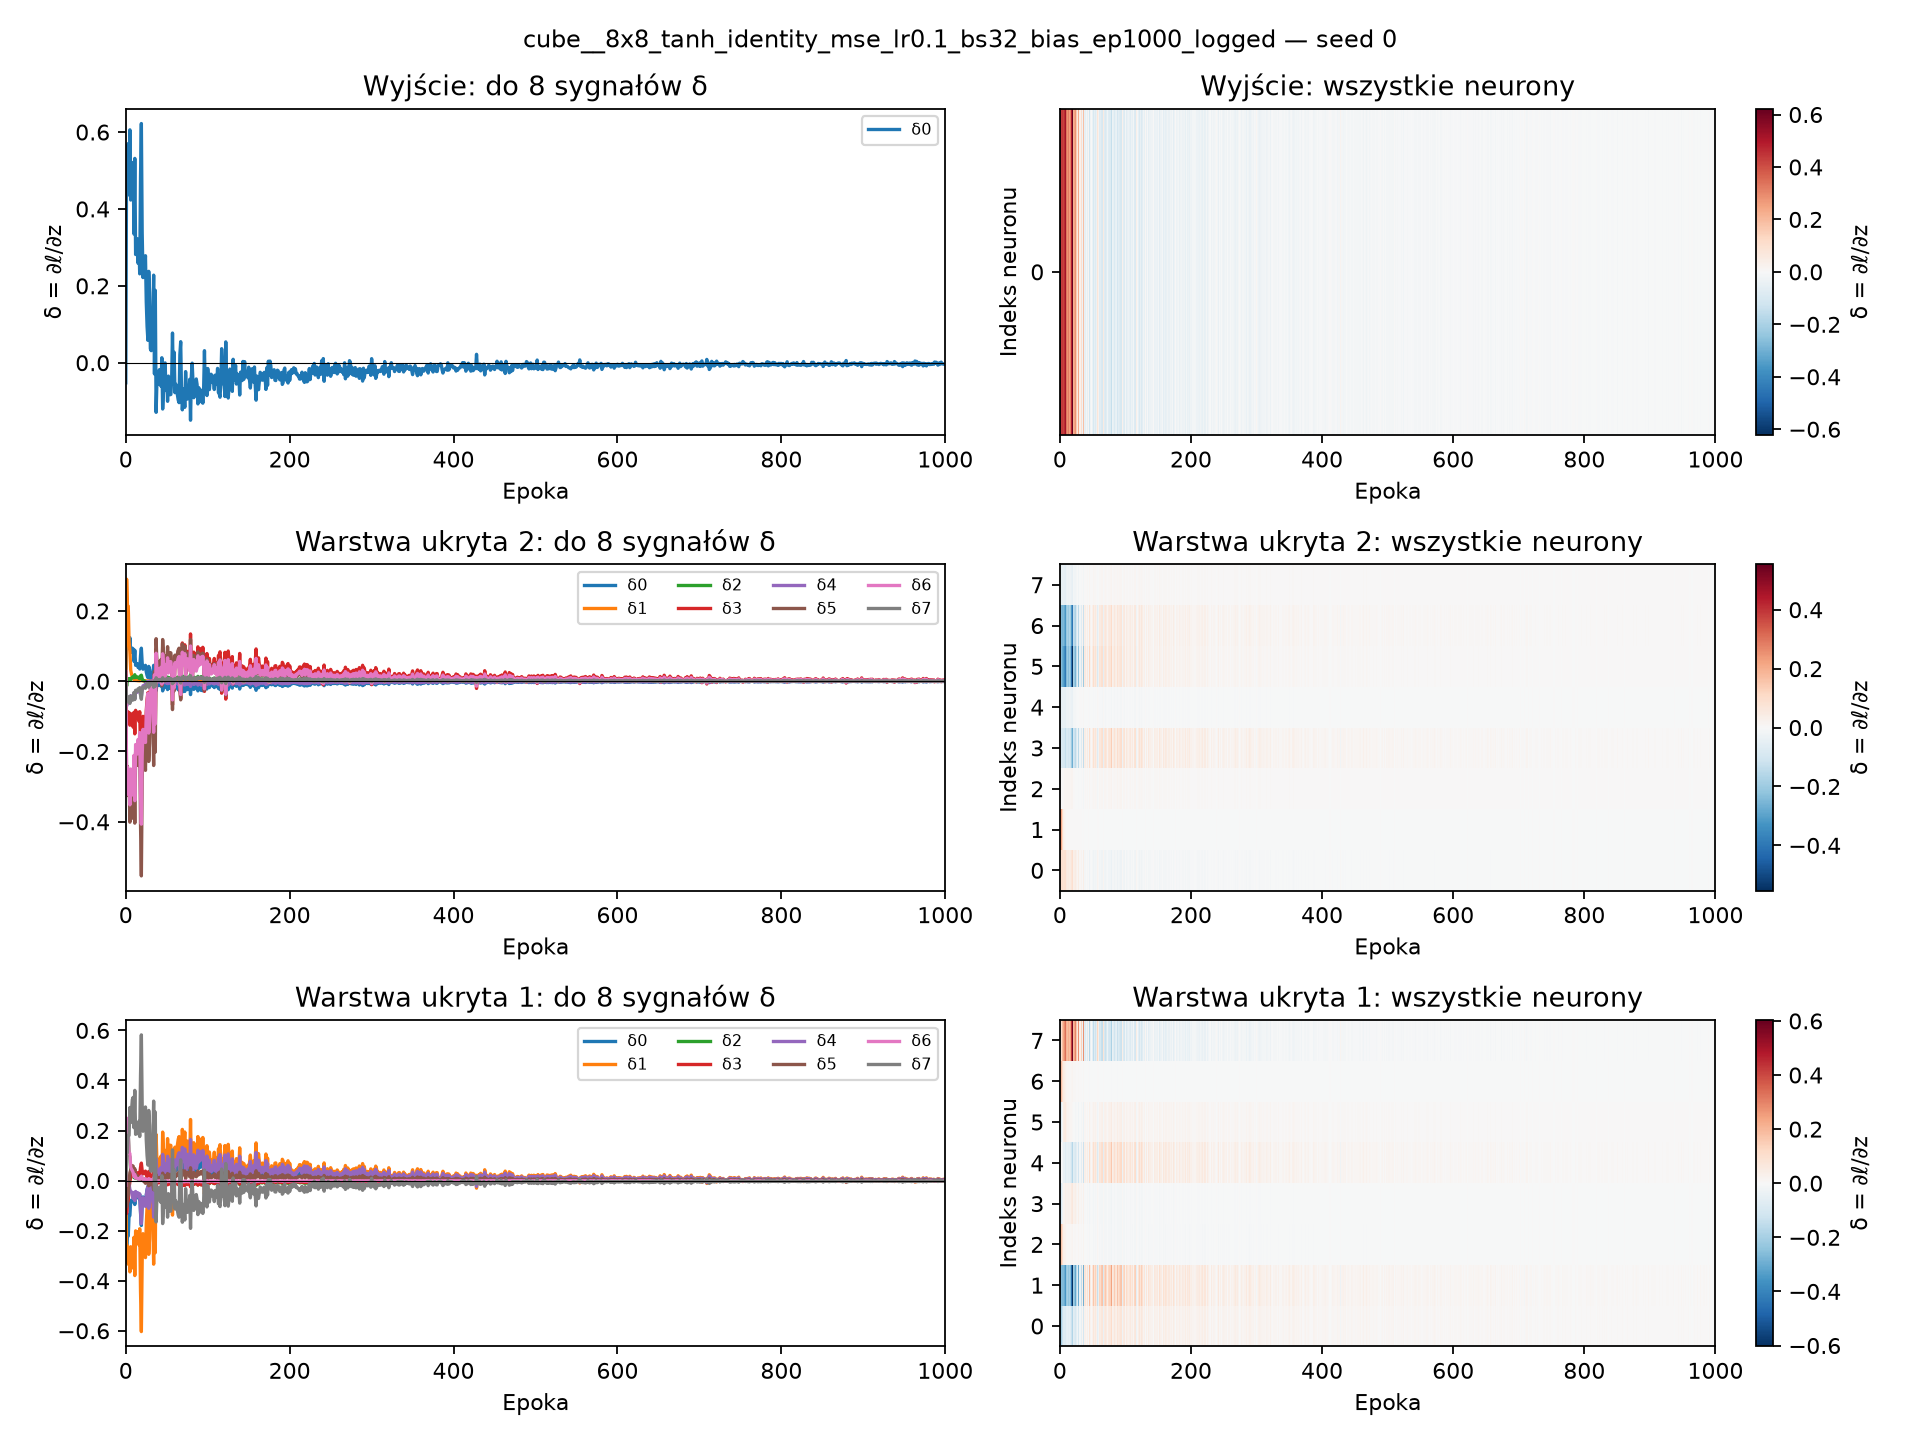
\includegraphics[width=\linewidth]{figures/single/cube__8x8_tanh_identity_mse_lr0.1_bs32_bias_ep1000_logged/seed_0/backpropagation.png}
  \caption{Błąd $\delta = \partial\mathcal{L}/\partial z$ propagowany wstecz od wyjścia (u góry)
  do pierwszej warstwy ukrytej (u dołu), dla ustalonego przykładu uczącego po każdej epoce
  (\emph{cube}, sieć $2\times8$, ziarno 0).}
  \label{fig:delty}
\end{figure}

\subsection{Architektura sieci}

Wyniki dla wszystkich architektur przedstawia rys.~\ref{fig:arch}. W klasyfikacji architektura ma
niewielki wpływ. Na \emph{simple} najlepsza jest sieć bez warstw ukrytych (99,6\%), a sieci głębsze
osiągają 99,1--99,5\%. Na \emph{three\_gauss} sieć liniowa osiąga 92,4\%, a każda sieć z warstwami
ukrytymi 93,3--93,7\%; sieci z~3--4 warstwami mają wyższą trafność na zbiorze uczącym niż testowym
(np.\ $4\times16$: 93,8\% wobec 93,4\%).

W regresji sieć bez warstw ukrytych nie jest w stanie dopasować funkcji (MSE 990 na \emph{cube}
i 707 na \emph{activation}), natomiast już jedna warstwa ukryta zmniejsza błąd o 3--5 rzędów
wielkości. Na \emph{cube} większość sieci z~2--4 warstwami osiąga MSE 0,2--0,9, wobec
1,0--1,7 dla jednej warstwy. Poza zakresem uczenia (rys.~\ref{fig:arch-out}) błąd na \emph{cube} rośnie z liczbą
warstw, a dla sieci z jedną warstwą maleje z jej szerokością.

\begin{figure}[htbp]
  \centering
  \begin{subfigure}{0.49\linewidth}
    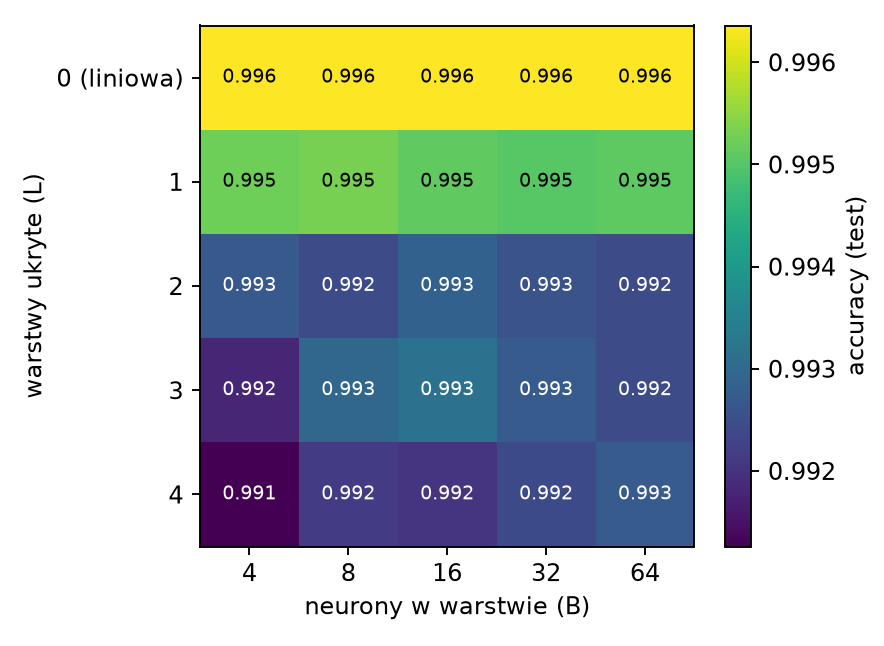
\includegraphics[width=\linewidth]{figures/simple/arch_heatmap_test_accuracy.png}
    \caption{\emph{simple}, accuracy}
  \end{subfigure}\hfill
  \begin{subfigure}{0.49\linewidth}
    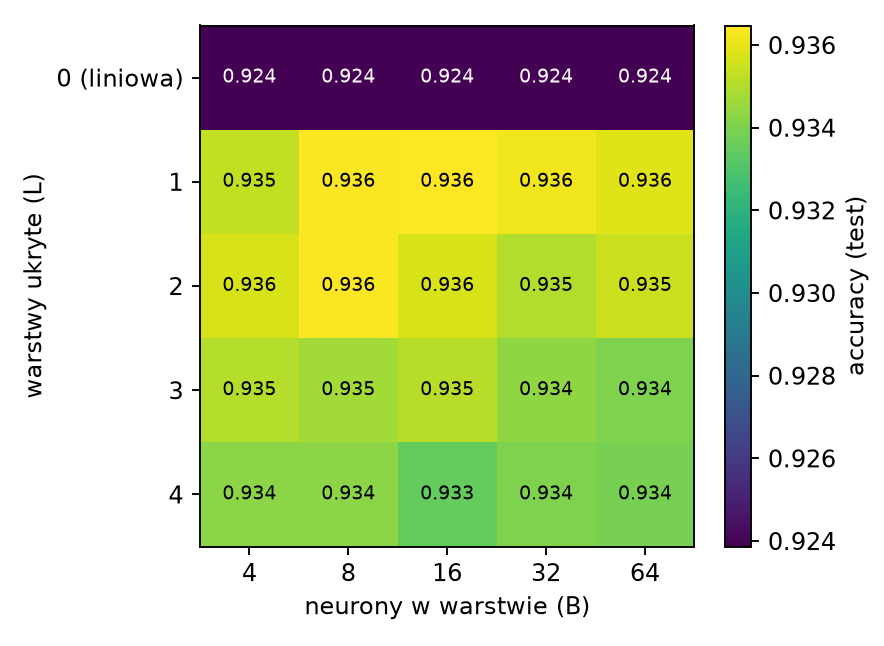
\includegraphics[width=\linewidth]{figures/three_gauss/arch_heatmap_test_accuracy.png}
    \caption{\emph{three\_gauss}, accuracy}
  \end{subfigure}
  \begin{subfigure}{0.49\linewidth}
    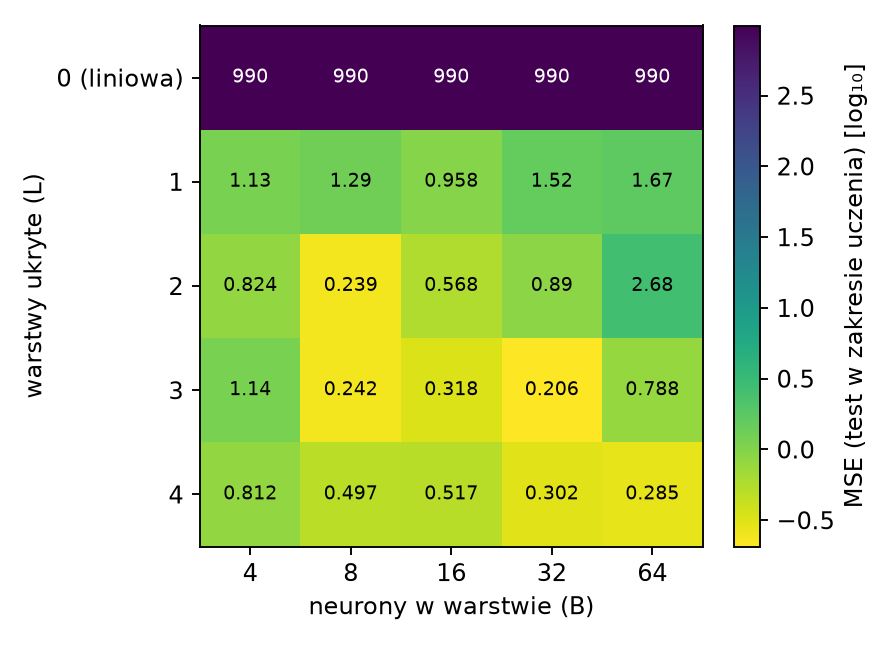
\includegraphics[width=\linewidth]{figures/cube/arch_heatmap_test_in_mse.png}
    \caption{\emph{cube}, MSE w zakresie uczenia}
  \end{subfigure}\hfill
  \begin{subfigure}{0.49\linewidth}
    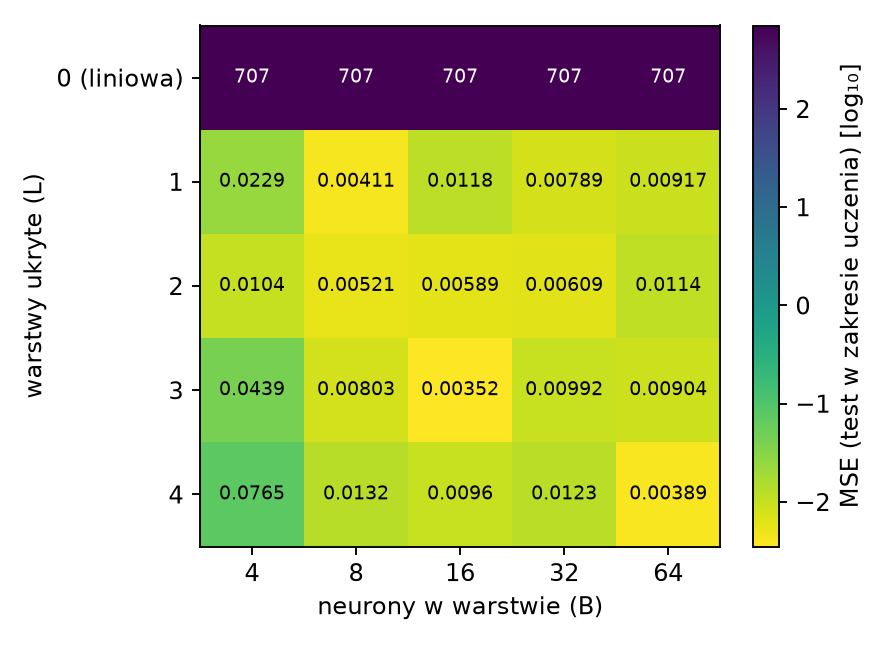
\includegraphics[width=\linewidth]{figures/activation/arch_heatmap_test_in_mse.png}
    \caption{\emph{activation}, MSE w zakresie uczenia}
  \end{subfigure}
  \caption{Wynik na zbiorze testowym w zależności od liczby warstw ukrytych $L$ i liczby neuronów
  w warstwie $B$ (mediana z 5 ziaren). W regresji kolor odpowiada $\log_{10}$ MSE.}
  \label{fig:arch}
\end{figure}

\begin{figure}[htbp]
  \centering
  \begin{subfigure}{0.49\linewidth}
    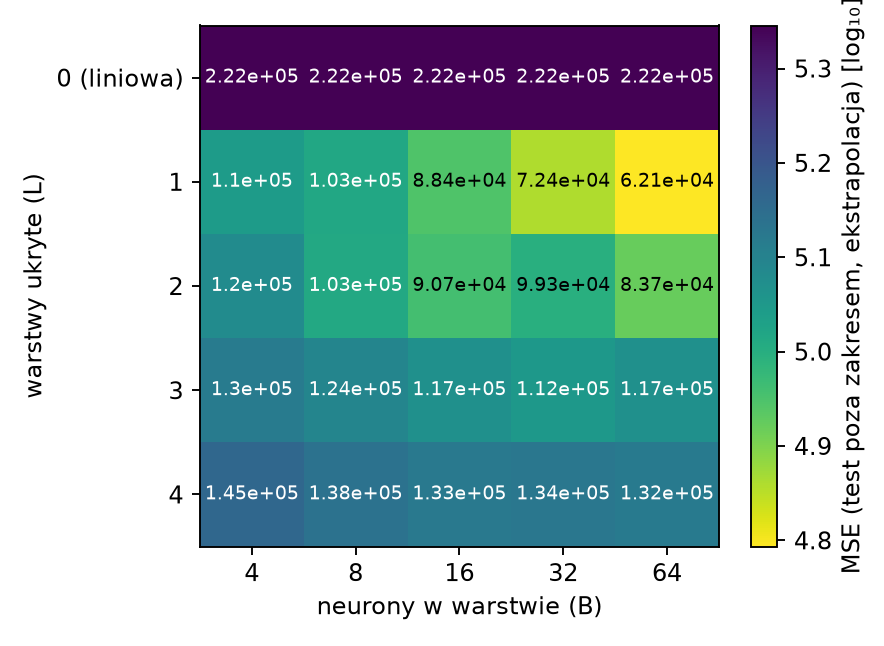
\includegraphics[width=\linewidth]{figures/cube/arch_heatmap_test_out_mse.png}
    \caption{\emph{cube}}
  \end{subfigure}\hfill
  \begin{subfigure}{0.49\linewidth}
    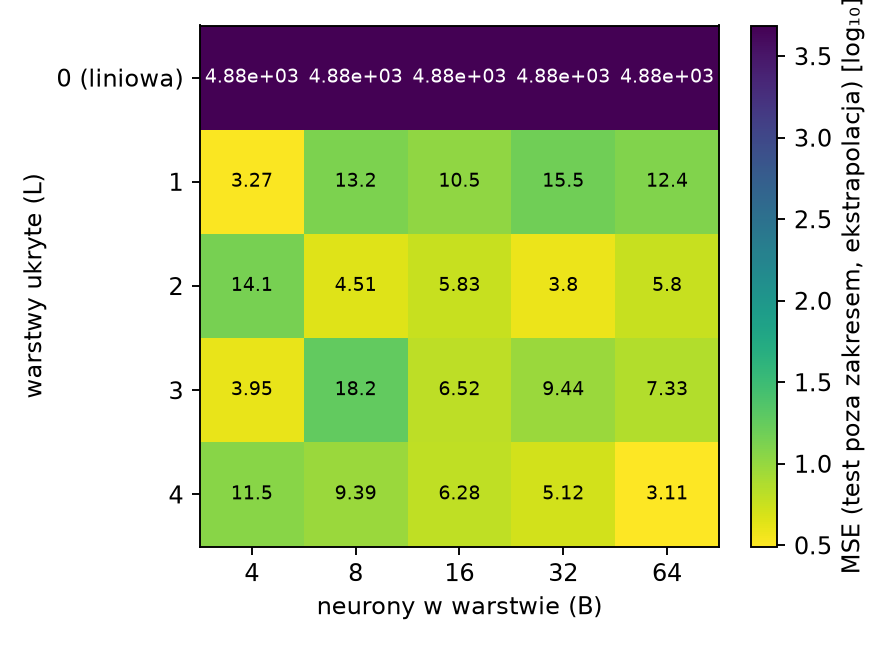
\includegraphics[width=\linewidth]{figures/activation/arch_heatmap_test_out_mse.png}
    \caption{\emph{activation}}
  \end{subfigure}
  \caption{MSE poza zakresem danych uczących w zależności od architektury.}
  \label{fig:arch-out}
\end{figure}

\subsection{Funkcja aktywacji}

Wpływ funkcji aktywacji silnie zależy od współczynnika uczenia (rys.~\ref{fig:aktywacja}).
Sigmoida wymaga największego kroku: na \emph{cube} osiąga MSE 0,61 przy współczynniku 0,3, a 241
przy 0,01, a na \emph{three\_gauss} jest najlepsza przy 0,3--1. $\tanh$ i ReLU osiągają najlepsze
wyniki przy mniejszych krokach, ale w regresji przy dużym kroku uczenie się rozbiega: przy
współczynniku 1 dla $\tanh$ we wszystkich ziarnach, dla ReLU w 3--5 ziarnach. Sigmoida nie
rozbiegła się w żadnym przypadku. Przy najlepszym kroku różnice między aktywacjami w klasyfikacji
nie przekraczają 0,3 p.p., natomiast w regresji są duże: na \emph{activation} $\tanh$ osiąga MSE
0,006, a sigmoida i ReLU ok.\ 0,25.

Funkcja aktywacji decyduje też o ekstrapolacji (rys.~\ref{fig:regresja}, \ref{fig:aktywacja-out}).
Na \emph{cube} najmniejszy błąd poza zakresem uczenia daje ReLU (MSE ok.\ $5\cdot10^4$ wobec ok.\
$10^5$ dla $\tanh$ i sigmoidy), a na \emph{activation} $\tanh$ (ok.\ 4 wobec 160--230 dla sigmoidy
i 1400--1800 dla ReLU).

\begin{figure}[htbp]
  \centering
  \begin{subfigure}{0.49\linewidth}
    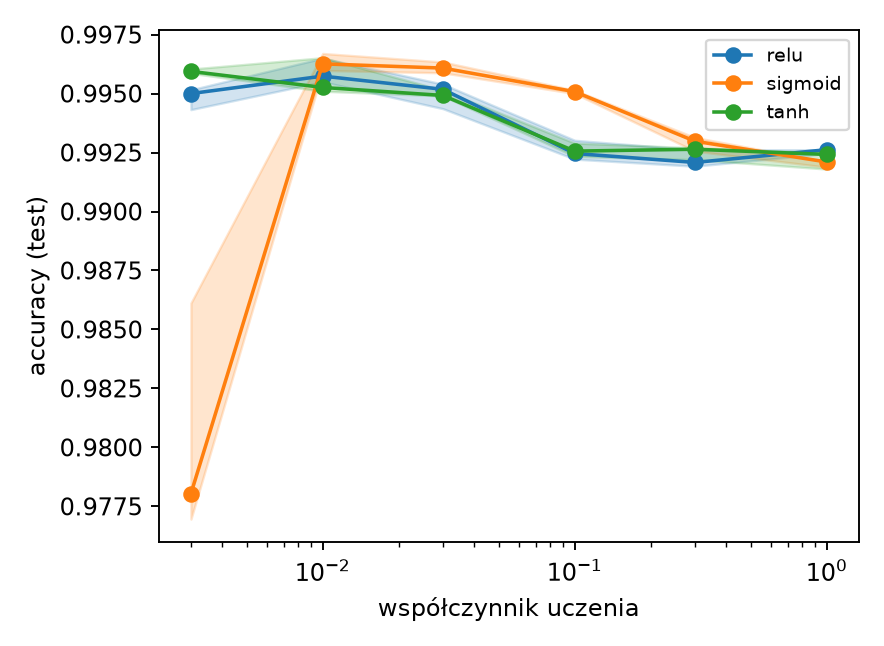
\includegraphics[width=\linewidth]{figures/simple/activation_lr_test_accuracy.png}
    \caption{\emph{simple}, accuracy}
  \end{subfigure}\hfill
  \begin{subfigure}{0.49\linewidth}
    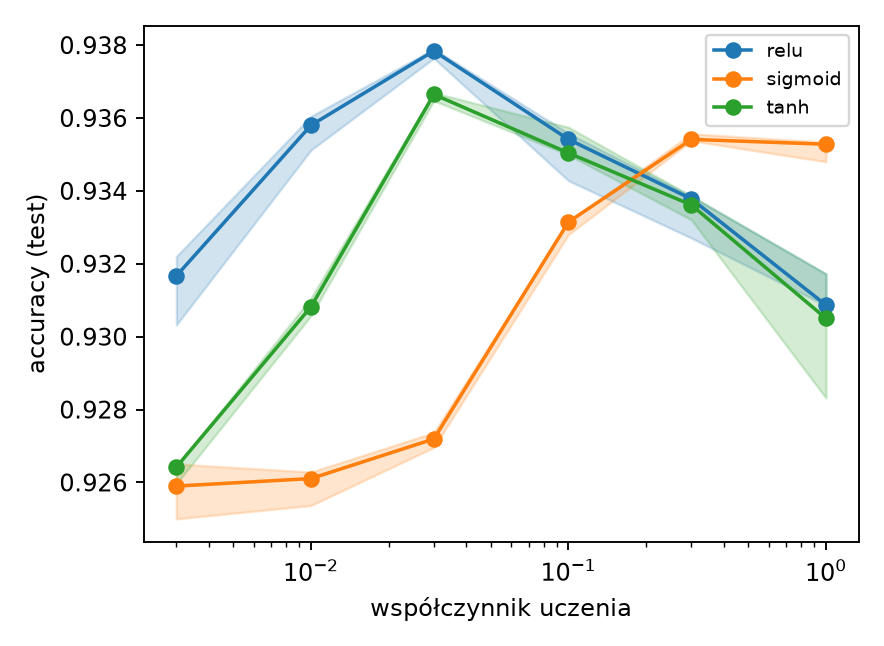
\includegraphics[width=\linewidth]{figures/three_gauss/activation_lr_test_accuracy.png}
    \caption{\emph{three\_gauss}, accuracy}
  \end{subfigure}
  \begin{subfigure}{0.49\linewidth}
    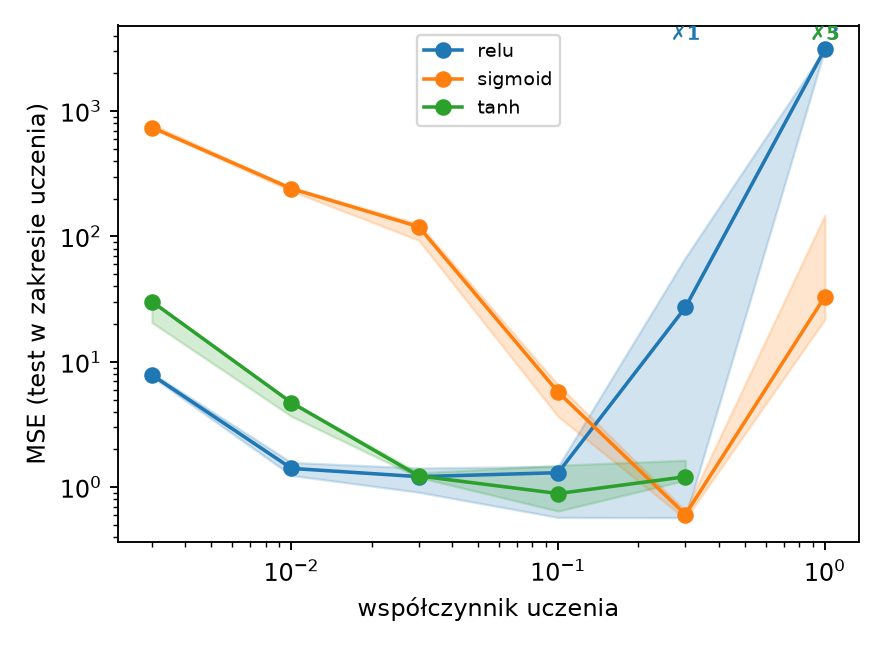
\includegraphics[width=\linewidth]{figures/cube/activation_lr_test_in_mse.png}
    \caption{\emph{cube}, MSE w zakresie uczenia}
  \end{subfigure}\hfill
  \begin{subfigure}{0.49\linewidth}
    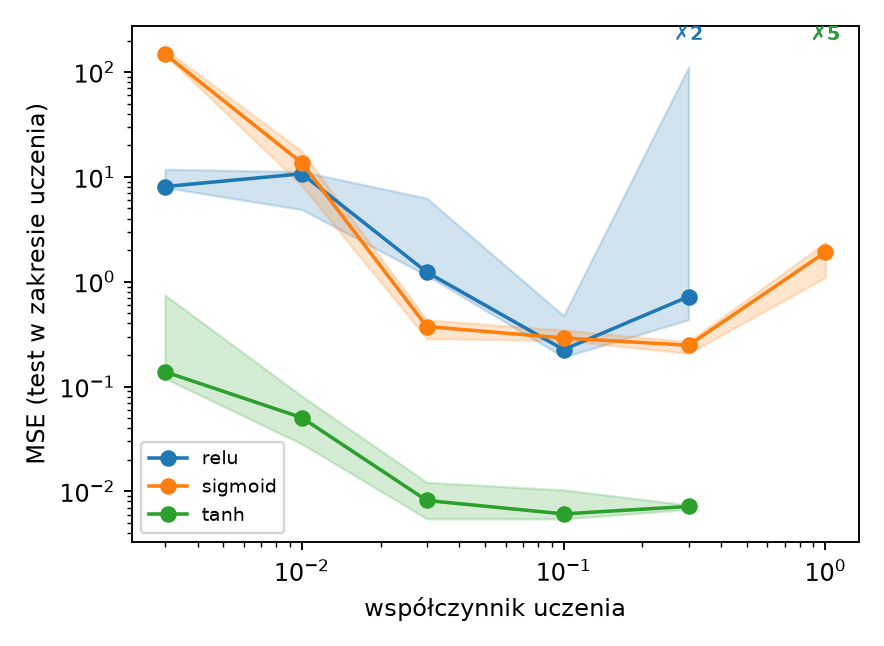
\includegraphics[width=\linewidth]{figures/activation/activation_lr_test_in_mse.png}
    \caption{\emph{activation}, MSE w zakresie uczenia}
  \end{subfigure}
  \caption{Funkcja aktywacji warstw ukrytych w zależności od współczynnika uczenia (sieć
  $2\times32$).}
  \label{fig:aktywacja}
\end{figure}

\begin{figure}[htbp]
  \centering
  \begin{subfigure}{0.49\linewidth}
    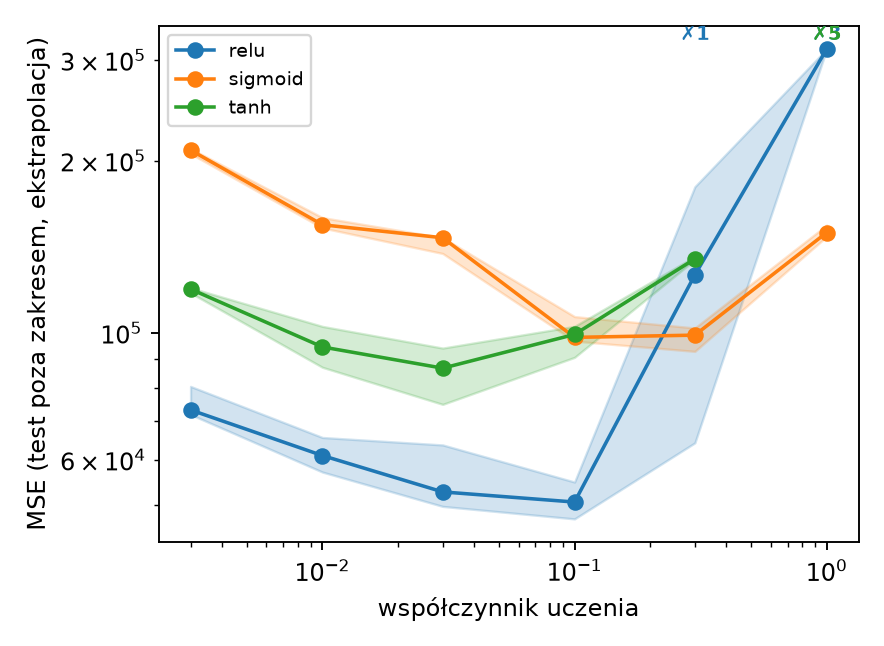
\includegraphics[width=\linewidth]{figures/cube/activation_lr_test_out_mse.png}
    \caption{\emph{cube}}
  \end{subfigure}\hfill
  \begin{subfigure}{0.49\linewidth}
    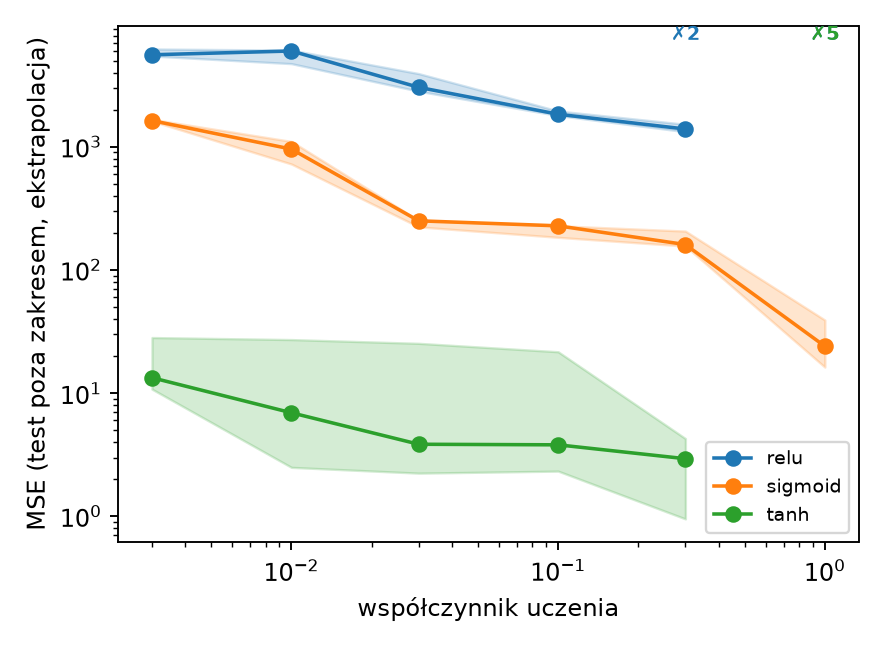
\includegraphics[width=\linewidth]{figures/activation/activation_lr_test_out_mse.png}
    \caption{\emph{activation}}
  \end{subfigure}
  \caption{MSE poza zakresem danych uczących dla różnych funkcji aktywacji.}
  \label{fig:aktywacja-out}
\end{figure}

\subsection{Funkcja kosztu}

W klasyfikacji (rys.~\ref{fig:koszt}a,b) MSE na wyjściu softmax wymaga większego kroku niż
entropia krzyżowa: na \emph{three\_gauss} najlepsze są odpowiednio współczynniki 0,1--0,3 i 0,03,
przy podobnej najlepszej trafności (93,6--93,7\%). Na \emph{simple} najlepsze wyniki obu
funkcji to 99,6--99,7\%.

W regresji (rys.~\ref{fig:koszt}c,d) koszt MAE daje gorsze wyniki niż MSE nawet w mierze MAE:
na \emph{cube} najlepsze MAE wynosi 2,1 przy uczeniu z kosztem MAE i 0,68 z kosztem MSE, na
\emph{activation} odpowiednio 0,68 i 0,07. Koszt MAE daje najlepsze wyniki przy najmniejszych
badanych krokach (0,003--0,01).

\begin{figure}[htbp]
  \centering
  \begin{subfigure}{0.49\linewidth}
    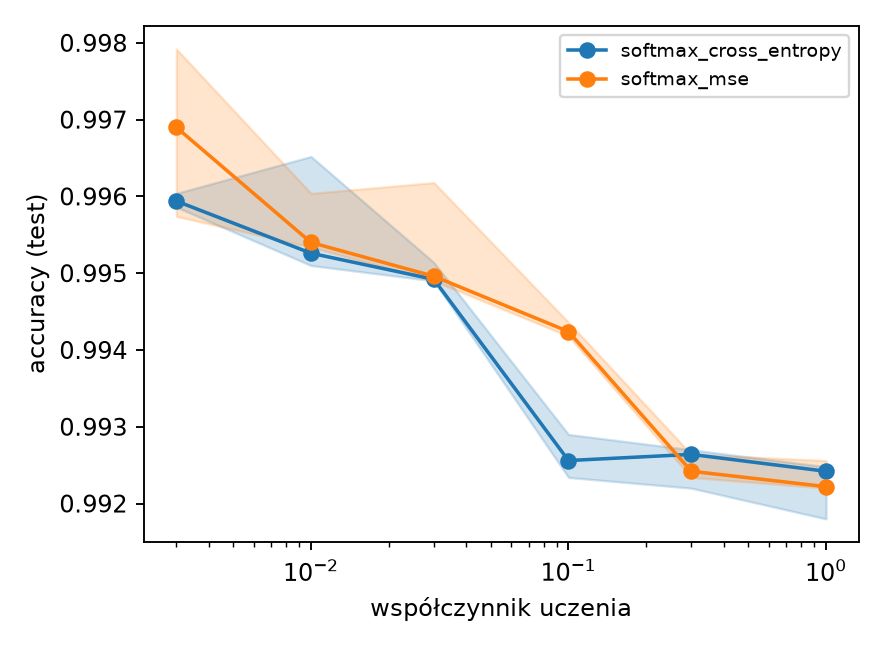
\includegraphics[width=\linewidth]{figures/simple/loss_lr_test_accuracy.png}
    \caption{\emph{simple}, accuracy}
  \end{subfigure}\hfill
  \begin{subfigure}{0.49\linewidth}
    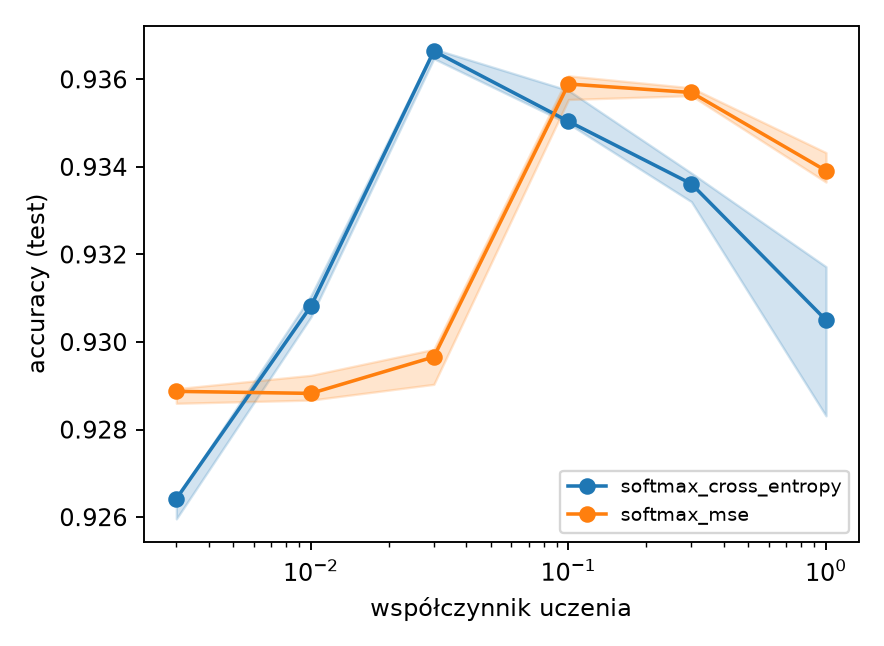
\includegraphics[width=\linewidth]{figures/three_gauss/loss_lr_test_accuracy.png}
    \caption{\emph{three\_gauss}, accuracy}
  \end{subfigure}
  \begin{subfigure}{0.49\linewidth}
    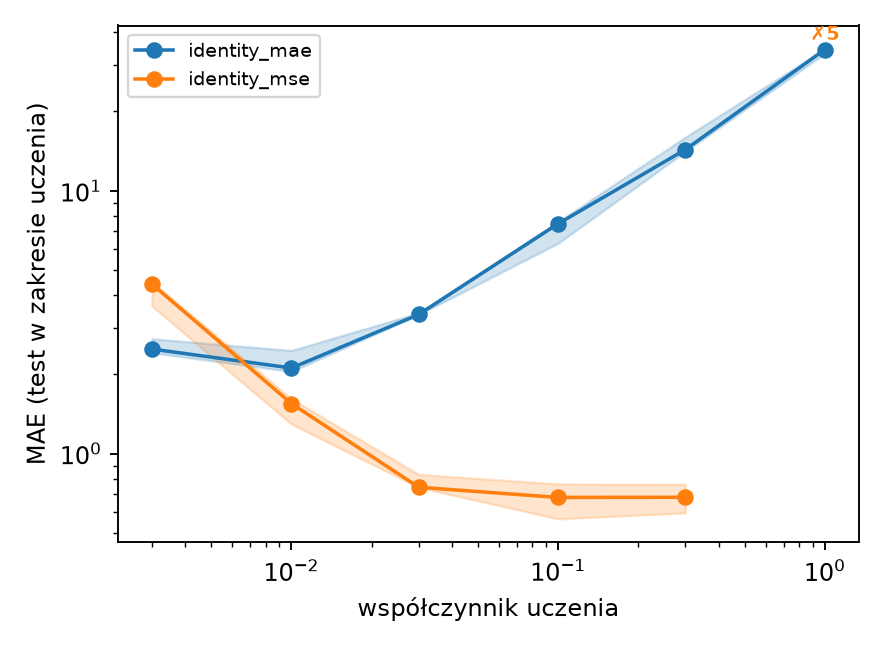
\includegraphics[width=\linewidth]{figures/cube/loss_lr_test_in_mae.png}
    \caption{\emph{cube}, MAE w zakresie uczenia}
  \end{subfigure}\hfill
  \begin{subfigure}{0.49\linewidth}
    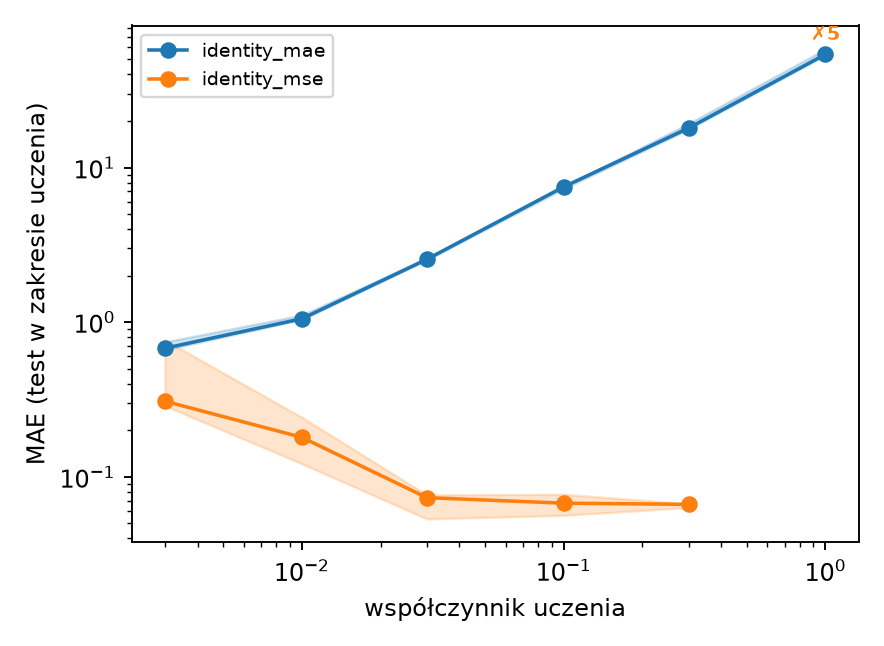
\includegraphics[width=\linewidth]{figures/activation/loss_lr_test_in_mae.png}
    \caption{\emph{activation}, MAE w zakresie uczenia}
  \end{subfigure}
  \caption{Funkcja kosztu w zależności od współczynnika uczenia (sieć $2\times32$, $\tanh$).}
  \label{fig:koszt}
\end{figure}

\subsection{Biasy}

Usunięcie biasów (rys.~\ref{fig:bias}) obniża trafność o 0,15--0,3 p.p.\ na \emph{simple} i o
1,1--1,4 p.p.\ na \emph{three\_gauss}. W regresji sieć bez biasów praktycznie nie uczy się funkcji:
MSE w zakresie uczenia wynosi 420--520 na \emph{cube} i ok.\ 660 na \emph{activation}, wobec
0,004--1,3 z biasami.

\begin{figure}[htbp]
  \centering
  \begin{subfigure}{0.49\linewidth}
    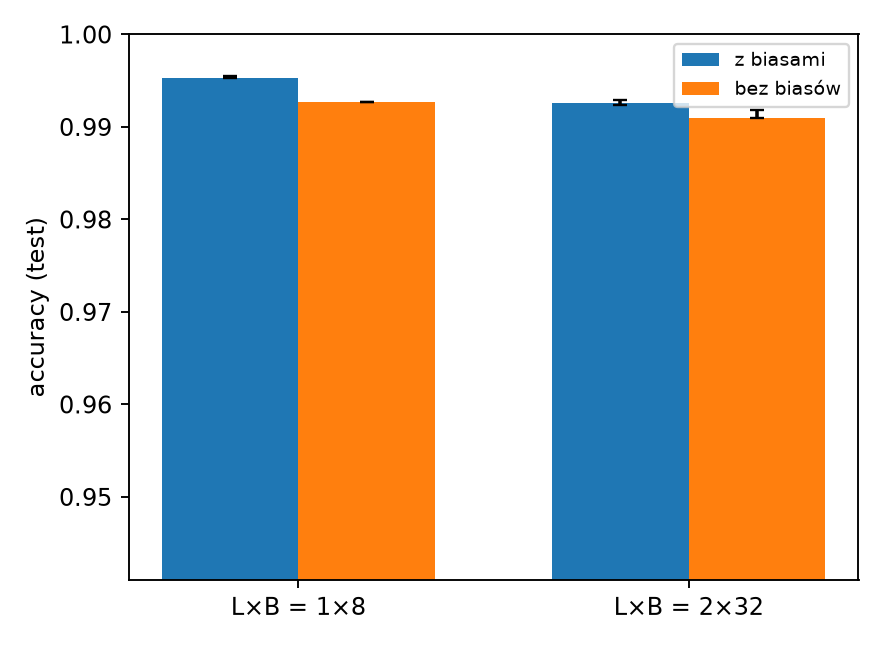
\includegraphics[width=\linewidth]{figures/simple/bias.png}
    \caption{\emph{simple}}
  \end{subfigure}\hfill
  \begin{subfigure}{0.49\linewidth}
    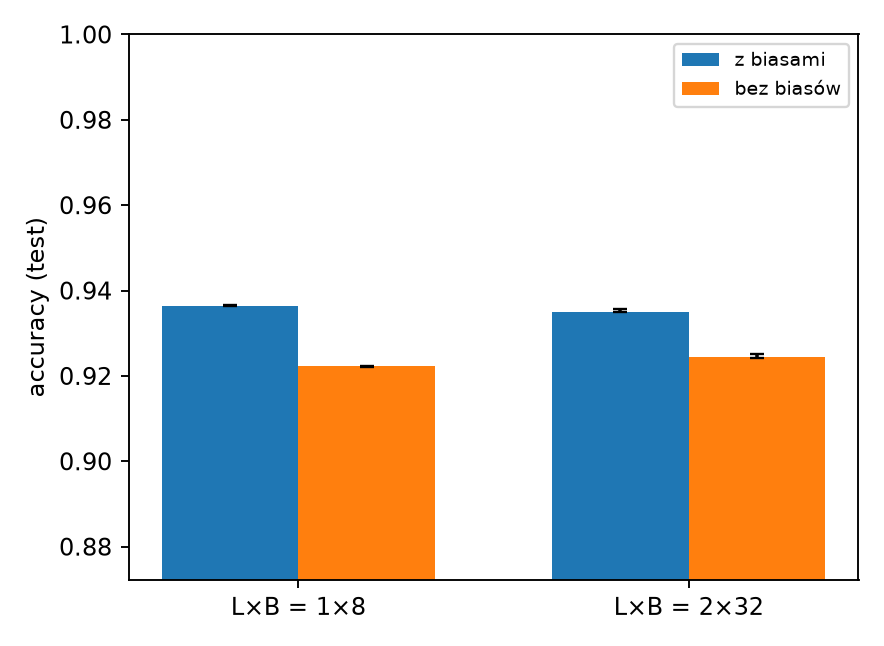
\includegraphics[width=\linewidth]{figures/three_gauss/bias.png}
    \caption{\emph{three\_gauss}}
  \end{subfigure}
  \begin{subfigure}{0.49\linewidth}
    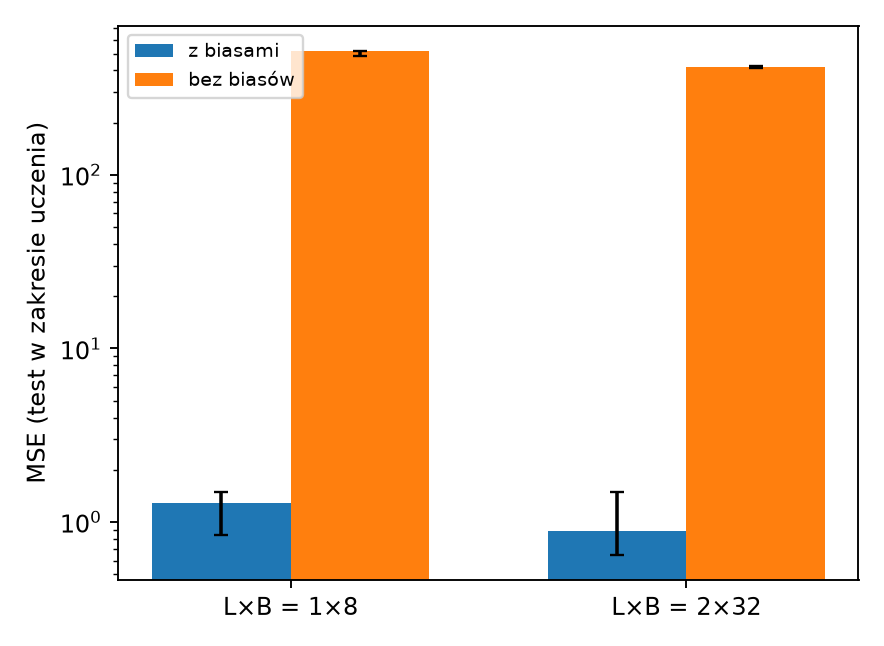
\includegraphics[width=\linewidth]{figures/cube/bias.png}
    \caption{\emph{cube}}
  \end{subfigure}\hfill
  \begin{subfigure}{0.49\linewidth}
    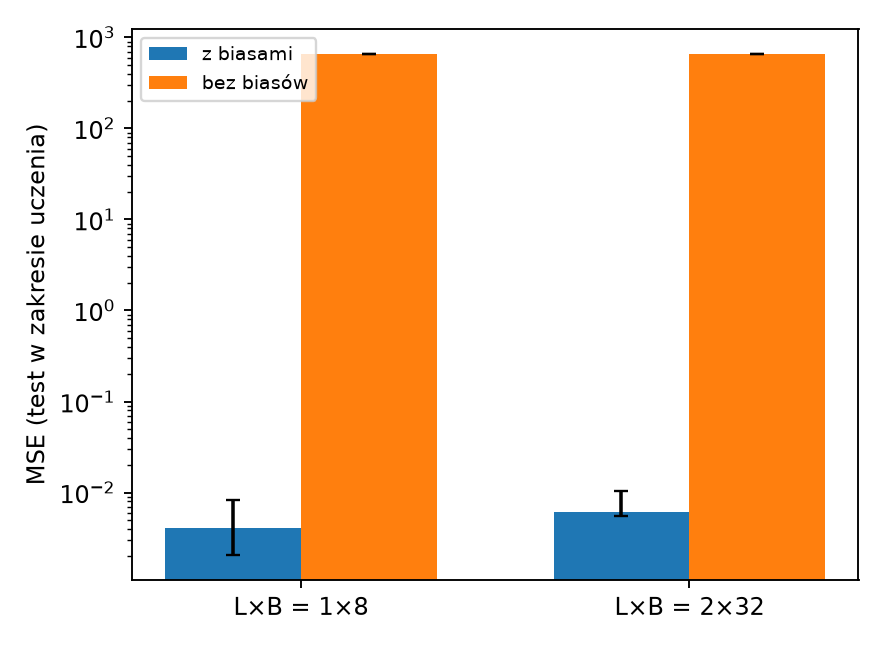
\includegraphics[width=\linewidth]{figures/activation/bias.png}
    \caption{\emph{activation}}
  \end{subfigure}
  \caption{Sieci $1\times8$ i $2\times32$ z biasami i bez biasów. W regresji MSE w zakresie
  uczenia (skala logarytmiczna).}
  \label{fig:bias}
\end{figure}

\section{Rozpoznawanie cyfr MNIST}
\label{sec:mnist}

\subsection{Dane i procedura}

Zbiór MNIST zawiera obrazy odręcznie pisanych cyfr 0--9 w skali szarości,
o rozmiarze $28\times28$ pikseli: 60\,000 uczących i 10\,000 testowych. Każdy obraz traktujemy jako
wektor 784 cech przeskalowanych do $[0,1]$, a sieć ma 10 wyjść z funkcją softmax. Program i
implementacja są te same co w części pierwszej; zmieniają się tylko parametry
(tab.~\ref{tab:mnist-baseline}).

Sieć uczy się wyłącznie na zbiorze uczącym. Zbiór testowy oceniamy po każdej epoce tylko w celu
zapisu wyników; nie wpływa on na uczenie ani na liczbę epok. Badania są analogiczne do części
pierwszej: architektura ($L \in \{0,1,2,3\}$, $B \in \{32, 128, 512\}$), funkcja aktywacji
i funkcja kosztu dla współczynników uczenia $\{0{,}01;\ 0{,}03;\ 0{,}1;\ 0{,}3\}$ oraz biasy (sieci
$1\times128$ i $2\times128$). Każdą konfigurację uczono z 5 ziarnami; wynik to średnia z ostatnich
5 epok, podawana jako mediana z ziaren.

\begin{table}[htbp]
\centering
\begin{tabular}{ll}
\toprule
warstwy ukryte & $1\times128$ \\
aktywacja warstw ukrytych & ReLU \\
wyjście i funkcja kosztu & softmax, entropia krzyżowa \\
biasy / inicjalizacja & tak / He, biasy zerowe \\
optymalizator & mini-batch SGD, batch 64 \\
współczynnik uczenia & 0,1 (stały) \\
liczba epok & 20 \\
normalizacja wejść & min-max do $[0,1]$ \\
precyzja obliczeń & 32-bitowa \\
\bottomrule
\end{tabular}
\caption{Konfiguracja bazowa dla MNIST.}
\label{tab:mnist-baseline}
\end{table}

\subsection{Architektura}

Trafność rośnie przede wszystkim z szerokością warstw (rys.~\ref{fig:mnist-arch},
tab.~\ref{tab:mnist-arch}): od 92,4\% dla sieci liniowej, przez 96,8\% ($1\times32$) i 97,8\%
($1\times128$), do 98,3\% dla $2\times512$. Druga warstwa ukryta daje niewielki zysk, trzecia
żaden. Sieci $2\times512$, $3\times128$ i $3\times512$ osiągają 100\% trafności na zbiorze
uczącym, a sieci z warstwami ukrytymi mają trafność na zbiorze uczącym o 1,4--2,0 p.p.\ wyższą niż
na testowym (sieć liniowa: 0,4 p.p., rys.~\ref{fig:mnist-krzywe}b). Koszt na zbiorze uczącym maleje przez całe uczenie, natomiast
koszt testowy po ok.\ 10 epokach prawie przestaje maleć (rys.~\ref{fig:mnist-krzywe}a).

\begin{figure}[htbp]
  \centering
  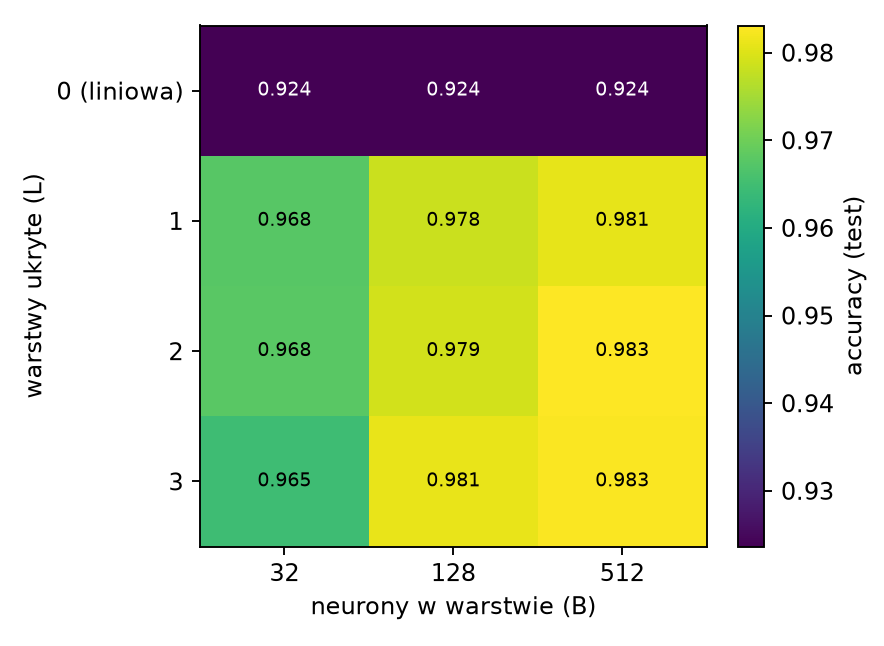
\includegraphics[width=0.6\linewidth]{figures/mnist/arch_heatmap_test_accuracy.png}
  \caption{MNIST: trafność na zbiorze testowym w zależności od liczby warstw ukrytych $L$ i liczby
  neuronów w warstwie $B$.}
  \label{fig:mnist-arch}
\end{figure}

\begin{table}[htbp]
  \centering
  \begin{tabular}{lrcc}
    \toprule
    architektura & liczba parametrów & accuracy (uczący) & accuracy (test) \\
    \midrule
    liniowa       & 7\,850   & 92,8\%  & 92,4\% \\
    $1\times32$   & 25\,450  & 98,1\%  & 96,8\% \\
    $1\times128$  & 101\,770 & 99,4\%  & 97,8\% \\
    $1\times512$  & 407\,050 & 99,8\%  & 98,1\% \\
    $2\times128$  & 118\,282 & 99,9\%  & 97,9\% \\
    $2\times512$  & 669\,706 & 100\%   & 98,3\% \\
    $3\times128$  & 134\,794 & 100\%   & 98,1\% \\
    $3\times512$  & 932\,362 & 100\%   & 98,3\% \\
    \bottomrule
  \end{tabular}
  \caption{MNIST: trafność wybranych architektur (mediana z 5 ziaren).}
  \label{tab:mnist-arch}
\end{table}

\begin{figure}[htbp]
  \centering
  \begin{subfigure}{0.49\linewidth}
    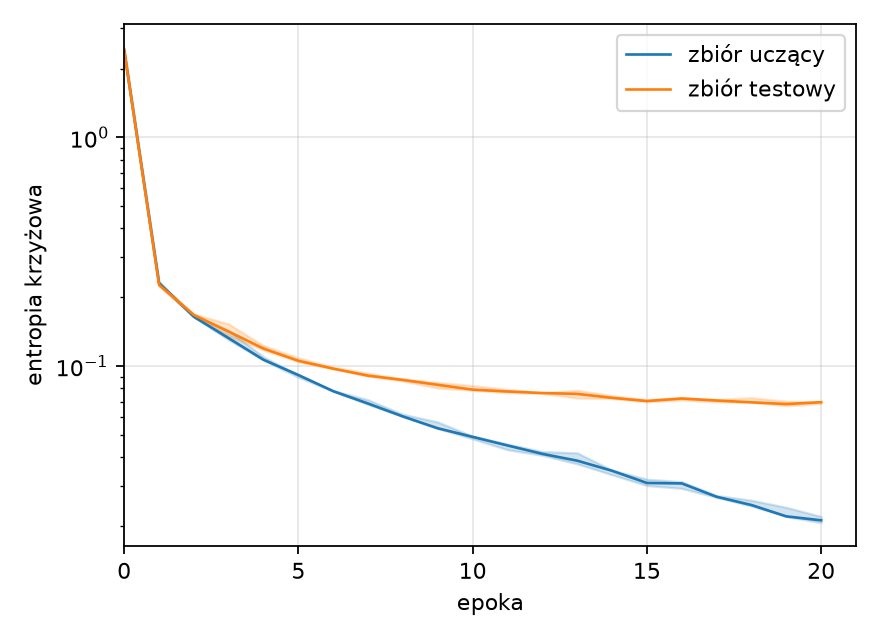
\includegraphics[width=\linewidth]{figures/mnist/cost_curve.png}
    \caption{koszt, sieć $1\times128$}
  \end{subfigure}\hfill
  \begin{subfigure}{0.49\linewidth}
    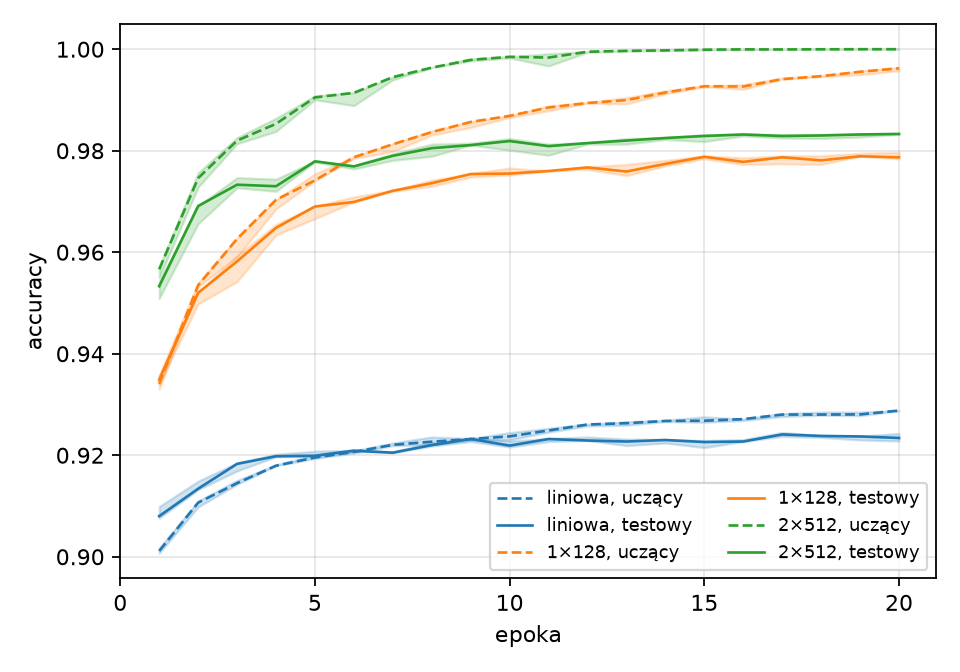
\includegraphics[width=\linewidth]{figures/mnist/arch_curves.png}
    \caption{trafność, trzy architektury}
  \end{subfigure}
  \caption{MNIST: przebieg uczenia na zbiorze uczącym i testowym (mediana i IQR z 5 ziaren).}
  \label{fig:mnist-krzywe}
\end{figure}

\subsection{Funkcja aktywacji i funkcja kosztu}

Dla wszystkich funkcji aktywacji trafność rośnie ze współczynnikiem uczenia w całym badanym zakresie
(rys.~\ref{fig:mnist-akt-koszt}a). Przy współczynniku 0,3 najlepsza jest ReLU (98,1\%), przed
$\tanh$ (97,9\%) i sigmoidą (97,5\%); przy współczynniku 0,01 przewaga ReLU nad sigmoidą wynosi
ok.\ 4 p.p. Entropia krzyżowa jest lepsza od MSE przy każdym badanym kroku
(rys.~\ref{fig:mnist-akt-koszt}b), o 2,7 p.p.\ przy współczynnikach 0,01--0,03 i o 0,5 p.p.\
przy 0,3.

\begin{figure}[htbp]
  \centering
  \begin{subfigure}{0.49\linewidth}
    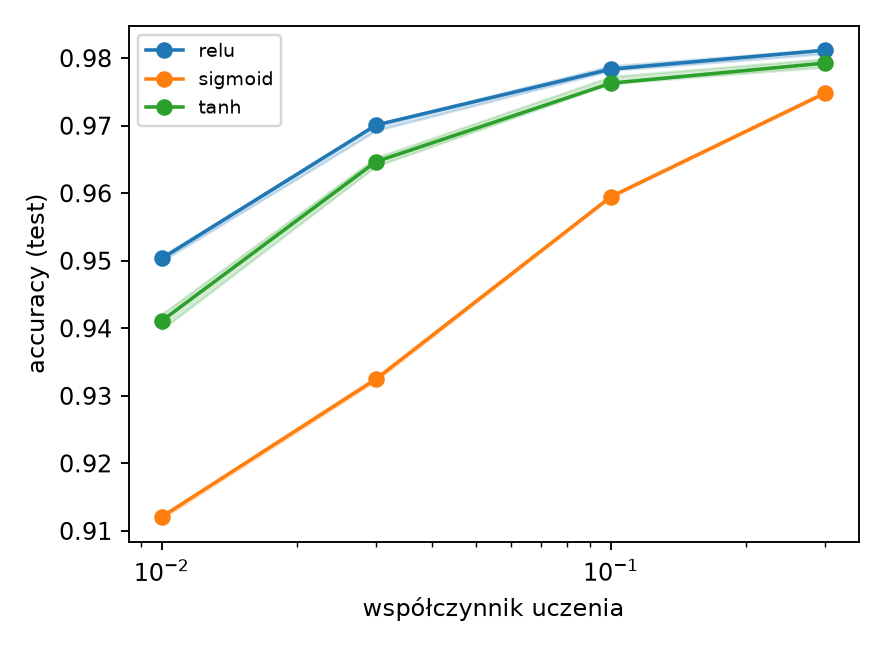
\includegraphics[width=\linewidth]{figures/mnist/activation_lr_test_accuracy.png}
    \caption{funkcja aktywacji}
  \end{subfigure}\hfill
  \begin{subfigure}{0.49\linewidth}
    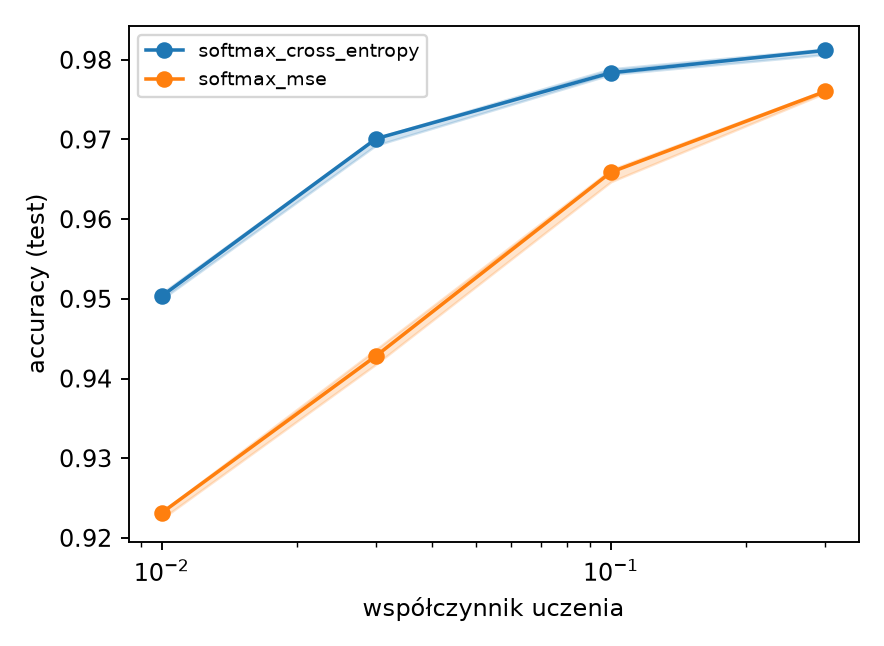
\includegraphics[width=\linewidth]{figures/mnist/loss_lr_test_accuracy.png}
    \caption{funkcja kosztu}
  \end{subfigure}
  \caption{MNIST: trafność na zbiorze testowym w zależności od współczynnika uczenia (sieć
  $1\times128$).}
  \label{fig:mnist-akt-koszt}
\end{figure}

\subsection{Biasy}

Na MNIST usunięcie biasów praktycznie nie zmienia wyniku (rys.~\ref{fig:mnist-bias}): trafność
sieci $1\times128$ wynosi 97,84\% z biasami i 97,81\% bez nich, a sieci $2\times128$ odpowiednio
97,90\% i 97,88\%. Różnice są mniejsze niż rozrzut między ziarnami.

\begin{figure}[htbp]
  \centering
  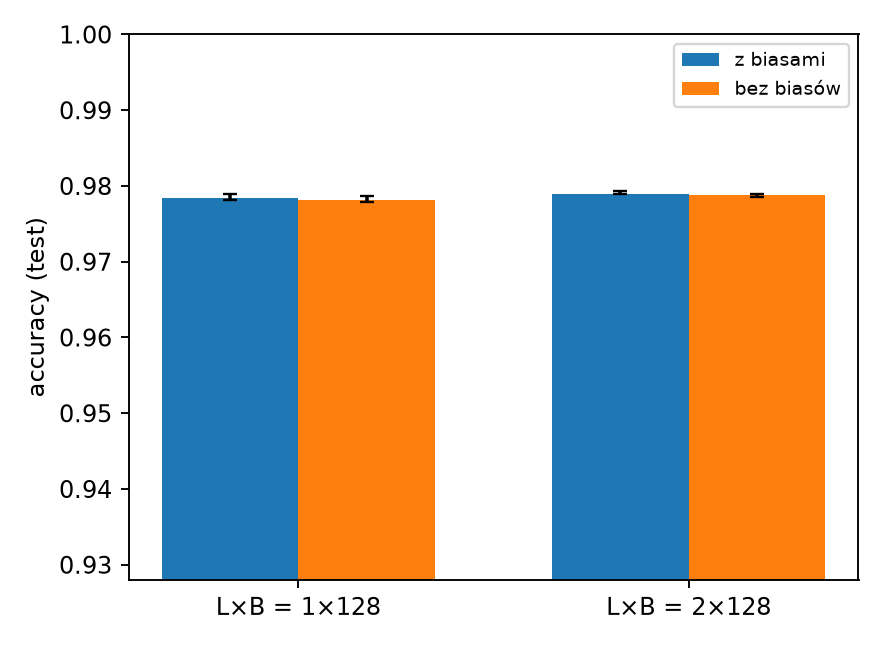
\includegraphics[width=0.55\linewidth]{figures/mnist/bias.png}
  \caption{MNIST: trafność na zbiorze testowym sieci z biasami i bez biasów.}
  \label{fig:mnist-bias}
\end{figure}

\subsection{Analiza błędów i wag}

Macierz pomyłek sieci bazowej (rys.~\ref{fig:mnist-pomylki}) pokazuje, że najczęściej mylone są
pary 4 i 9 (po 46 przypadków w obie strony, sumarycznie dla 5 ziaren), 2 i 7 oraz cyfry 5 i 8
z cyfrą 3. Najlepiej rozpoznawane są cyfry 0 i 1 (ok.\ 99\%), najsłabiej 5, 8 i 9 (ok.\ 97\%).

\begin{figure}[htbp]
  \centering
  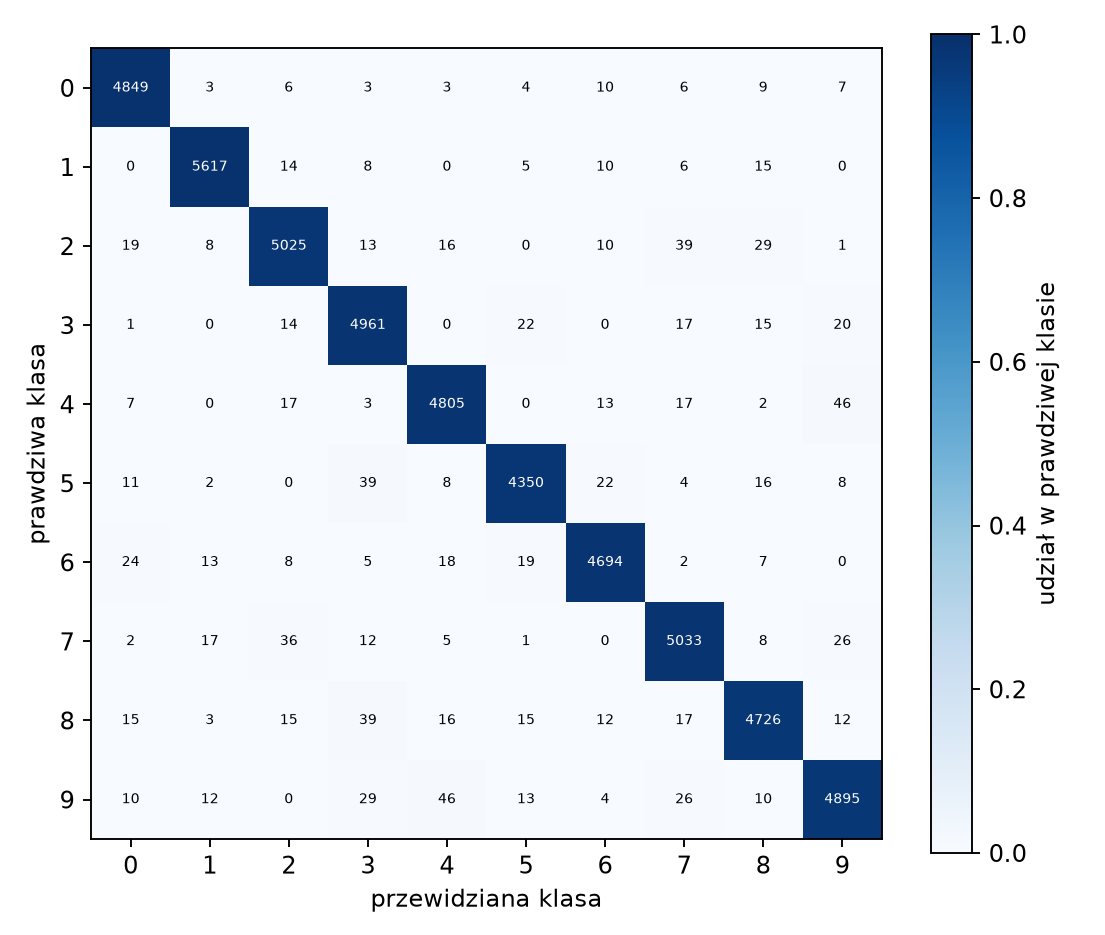
\includegraphics[width=0.6\linewidth]{figures/mnist/confusion_relu_128.png}
  \caption{MNIST: macierz pomyłek sieci bazowej na zbiorze testowym po ostatniej epoce,
  zsumowana po 5 ziarnach.}
  \label{fig:mnist-pomylki}
\end{figure}

Rysunek~\ref{fig:mnist-wagi} przedstawia wagi pierwszej warstwy jako obrazy $28\times28$.
Po pierwszej epoce zmiany wag tworzą gładkie wzory w środkowej części obrazu, w której leżą cyfry,
a wagi pikseli brzegowych prawie się nie zmieniają. Niektóre wzory przypominają fragmenty cyfr,
np.\ ukośną kreskę. Po 20 epokach wzory są drobniejsze i mniej regularne.

\begin{figure}[htbp]
  \centering
  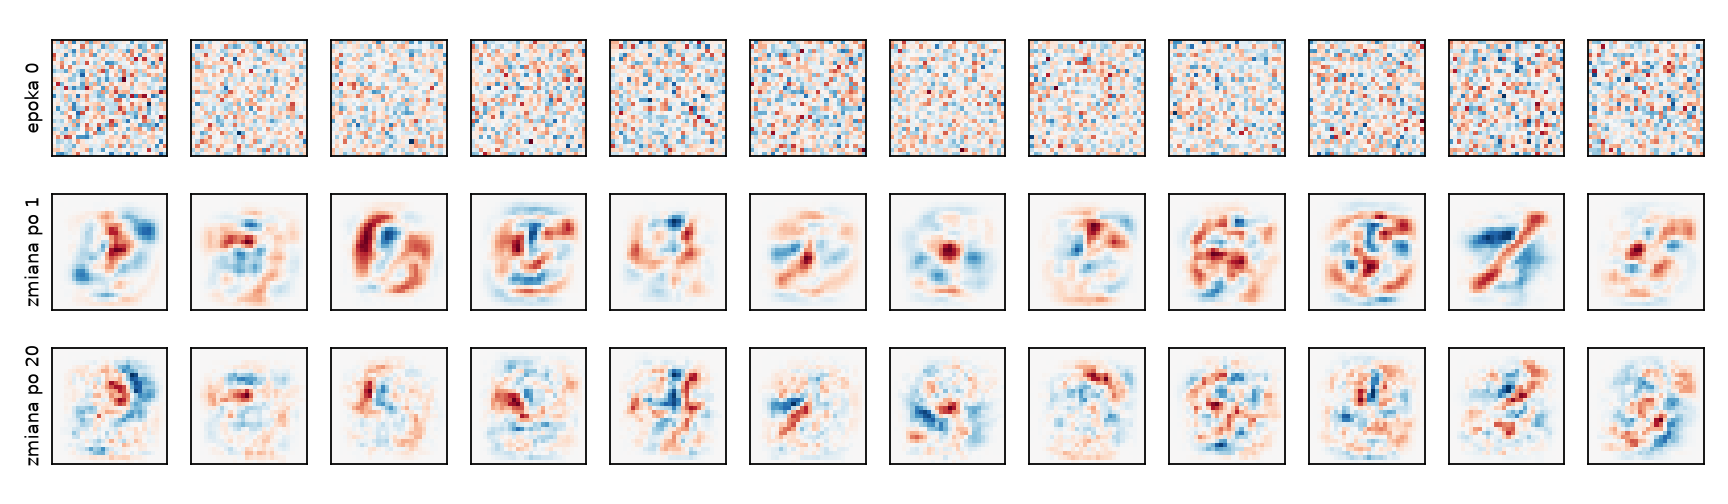
\includegraphics[width=\linewidth]{figures/mnist/weights_tiles.png}
  \caption{MNIST: wagi 12 pierwszych neuronów warstwy ukrytej sieci $1\times128$ (ziarno 0)
  przedstawione jako obrazy $28\times28$: wartości początkowe oraz ich zmiana po pierwszej
  i po ostatniej epoce (czerwony -- dodatnie, niebieski -- ujemne, każdy obraz we własnej skali).}
  \label{fig:mnist-wagi}
\end{figure}



\section{Podsumowanie i wnioski}
\label{sec:wnioski}

Zaimplementowana sieć MLP poprawnie rozwiązuje zadania klasyfikacji i regresji, a wyniki
są powtarzalne: rozrzut między ziarnami jest mały, a uczenie rozbiegało się tylko w regresji
przy największych współczynnikach uczenia. Z przeprowadzonych badań wynika, że:
\begin{itemize}
  \item w regresji konieczna jest co najmniej jedna warstwa ukryta, natomiast w prostych
  zadaniach klasyfikacji w $\mathbb{R}^2$ warstwy ukryte dają niewielki zysk; dodatkowe warstwy
  dają niewielki zysk w zakresie danych uczących i pogarszają ekstrapolację,
  \item wpływ funkcji aktywacji zależy od współczynnika uczenia: sigmoida wymaga większego kroku,
  ale jest stabilna, a $\tanh$ i ReLU osiągają dobre wyniki przy mniejszym kroku, lecz przy dużym kroku mogą się rozbiegać;
  poza zakresem danych uczących sieć przejmuje kształt funkcji aktywacji,
  \item w klasyfikacji entropia krzyżowa daje lepsze lub podobne wyniki niż MSE przy mniejszym
  kroku, a w regresji MSE jest lepsze od MAE, także w mierze MAE,
  \item biasy są niezbędne w regresji i poprawiają klasyfikację w $\mathbb{R}^2$, natomiast na
  MNIST nie mają zauważalnego wpływu,
  \item na MNIST najlepszą trafność (98,3\%) osiąga sieć z dwiema warstwami po 512 neuronów;
  szerokość warstw ma większy wpływ niż ich liczba, a największe sieci dopasowują się
  w całości do zbioru uczącego.
\end{itemize}

\begin{thebibliography}{9}
\addcontentsline{toc}{section}{Literatura}

\bibitem{glorot2010}
X.~Glorot, Y.~Bengio, \emph{Understanding the difficulty of training deep feedforward neural
networks}, AISTATS, 2010.

\bibitem{he2015}
K.~He, X.~Zhang, S.~Ren, J.~Sun, \emph{Delving Deep into Rectifiers: Surpassing Human-Level
Performance on ImageNet Classification}, ICCV, 2015.

\end{thebibliography}

\end{document}
